\documentclass[11pt]{article}
\usepackage{ifthen}
\newboolean{overleaf}\setboolean{overleaf}{false} % set to true for compatibility with overleaf
\newboolean{draft}\setboolean{draft}{true} % whether to display notes (e.g. TODO, FIXME, etc)
\newboolean{gitinfo}\setboolean{gitinfo}{true} % whether use gitinfo2 to provide git detail (doesn't work in Overleaf; you may also need to run setup.sh the first time)
\ifthenelse{\boolean{overleaf}}{\setboolean{gitinfo}{false}}{}

\usepackage[truedimen, top=2cm,bottom=2cm,left=2cm,right=2cm]{geometry}
\geometry{a4paper} 
%\usepackage[parfill]{parskip}    % Activate to begin paragraphs with an empty line rather than an indent
\ifthenelse{\boolean{overleaf}}{\usepackage[demo]{graphicx}}{\usepackage{graphicx}}
\usepackage{amssymb}
%\usepackage{epstopdf}
%\DeclareGraphicsRule{.tif}{png}{.png}{`convert #1 `dirname #1`/`basename #1 .tif`.png}

\usepackage[table,dvipsnames]{xcolor}    % loads also colortbl
\definecolor{lightblue}{rgb}{0.93,0.95,1.0}
%%\rowcolors{2}{blue!4}{white}
%\rowcolors{1}{lightblue}{white}
\definecolor{link}{rgb}{0,0,1}
\usepackage[colorlinks,
linkcolor={link},citecolor={link},urlcolor={link},
 breaklinks, bookmarks, bookmarksopen, bookmarksnumbered
]{hyperref}
\usepackage{url}\urlstyle{sf} % rm, sf, tt or same
%% Define a new style for the urls that will use a smaller font.
\makeatletter
\def\url@smallurlstyle{%
  \@ifundefined{selectfont}{\def\UrlFont{\sf}}{\def\UrlFont{\footnotesize\sffamily}}}
\makeatother
%% Now actually use the newly defined style.
\urlstyle{smallurl}

\usepackage{PTSansNarrow} % narrow sans serif font for urls
\usepackage[scaled=.9]{inconsolata} % for texttt
\usepackage{mathpazo}

\usepackage{tikz}
\tikzset{
    state/.style={
           rectangle,
           rounded corners,
           draw=black, ultra thick,
           minimum height=2em,
           inner sep=2pt,
           text centered,
           text width=40ex
           },
}

\usepackage{datetime2}\DTMsetdatestyle{iso}
\ifthenelse{\boolean{gitinfo}}{\usepackage[grumpy]{gitinfo2}}{}
\usepackage{qrcode}
\usepackage{natbib}
\usepackage{ltablex}\keepXColumns
\usepackage{sistyle} % TODO: replace with siunitx?
%\usepackage{siunitx} % would need to update nmltab to replace \num* with the siunitx equivalent
\usepackage{array}
\usepackage[strings]{underscore} % allows hyphenation at underscores
\usepackage[nooneline,small,hypcap=true]{caption} % correct hypcap needs v 3.1 or higher
\renewcommand{\captionlabelfont}{\bfseries}
\setlength{\captionmargin}{0.5cm} \setlength{\abovecaptionskip}{3pt}
\usepackage{placeins}

\ifthenelse{\boolean{draft}}
{\newcommand{\note}[1]{#1}} % show all notes
{\newcommand{\note}[1]{\quad}} % hide all notes

\newcommand{\TODO}[1]{\note{\textcolor{blue}{\textsf{\textbf{TODO: #1}}}}}
\newcommand{\FIXME}[1]{\note{\textcolor{red}{\textsf{\textbf{FIXME: #1}}}}}
\newcommand{\CONTRIBUTORS}[1]{\note{\textcolor{BurntOrange}{\textsf{\textsl{CONTRIBUTORS: #1}}}}}
\newcommand{\ISSUE}[1]{\note{\colorbox{yellow}{\textsf{\textbf{\href{https://github.com/OceansAus/ACCESS-OM2-1-025-010deg-report/issues/#1}{ISSUE #1}}}}}}
\newcommand{\CISSUE}[1]{\note{\colorbox{gray}{\textsf{\textbf{\href{https://github.com/OceansAus/ACCESS-OM2-1-025-010deg-report/issues/#1}{ISSUE #1}}}}}}
\setlength{\fboxsep}{0pt} 
% link directly to github source
%\newcommand{\momlink}[2]{\href{https://github.com/mom-ocean/MOM5/search?q=#2}{#1}}
%\newcommand{\cicelink}[2]{\href{https://github.com/OceansAus/cice5/search?q=#2}{#1}}
%\newcommand{\yatmlink}[2]{\href{https://github.com/OceansAus/libaccessom2/search?q=#2}{#1}}
% link to appendix tables 
% need work around to handle names that include _   (which is many of them!)  - possibly due to use of underscore package?
% derived from https://tex.stackexchange.com/questions/129739/label-and-non-plain-text-arguments
\makeatletter
\newcommand*{\make@hex@label}[1]{%
  \def\hex@label{#1}%
  \@onelevel@sanitize\hex@label
  \EdefEscapeHex\hex@label{\hex@label}%
}
\newcommand*{\hexhypertarget}[2]{%
  \@bsphack
    \make@hex@label{#1}%
    \hypertarget{\hex@label}{#2}%
  \@esphack
}
\newcommand*{\hexhyperlink}[2]{%
  \make@hex@label{#1}%
  \hyperlink{\hex@label}{#2}%
}
\makeatother
\newcommand{\momlink}[2]{\hexhyperlink{mom:#2}{#1}}
\newcommand{\cicelink}[2]{\hexhyperlink{cice:#2}{#1}}
\newcommand{\yatmlink}[2]{\hexhyperlink{yatm:#2}{#1}}
% can \StrSubstitute in xstring be used to remove _? - can't get this to work
%\usepackage{xstring}
%\newcommand{\momlink}[2]{\hyperlink{mom:#2}{#1 mom:\StrSubstitute{#2}{_}{}}}
%\newcommand{\momlink}[2]{\hyperlink{mom:\StrSubstitute{#2}{_}{_}}{#1 mom:\StrSubstitute{#2}{_}{}}}

\newcommand{\param}[1]{\textsf{#1}}
\newcommand{\mom}[1]{\param{\momlink{#1}{#1}}}
\newcommand{\cice}[1]{\param{\cicelink{#1}{#1}}}
\newcommand{\yatm}[1]{\param{\yatmlink{#1}{#1}}}

\newcommand{\nmldiffer}[1]{#1} % no special display of differing variables
%\newcommand{\nmldiffer}[1]{\textbf{#1}} % bold display of differing variables
%\definecolor{hilite}{cmyk}{0, 0, 0.9, 0}\newcommand{\nmldiffer}[1]{\colorbox{hilite}{#1}}\setlength{\fboxsep}{0pt} % colour highlight of differing variables (requires color package)
\newcommand{\nmllink}[2]{#1} % don't link variables
% \newcommand{\nmllink}[2]{\href{https://github.com/mom-ocean/MOM5/search?q=#2}{#1}} % link variables to documentation (requires hyperref package)
\definecolor{ignore}{gray}{0.7}\newcommand{\ignored}[1]{\textcolor{ignore}{#1}} % gray display of ignored variables (requires color package)
%\newcommand{\nml}[1]{{\small\textsf{\input{local/#1}}}}
\newcommand{\nml}[1]{{\footnotesize\textsf{\input{#1}}}}
\newlength{\nmllen}\setlength{\nmllen}{8ex}
%\newcommand{\doscript}[1]{\texttt{#1}\\{\footnotesize\textsf{\input{|"#1"}}}}
\newcommand{\doscript}[1]{{\footnotesize\textsf{\input{|"#1"}}}}
%\newcommand{\doscript}[1]{{\footnotesize\textsf{\input{|"#1 > tmp.tex"}\input{tmp.tex}}}}
\newcommand{\runchanges}[1]{\subsection{#1}%
%\renewcommand{\nmllink}[2]{\href{https://github.com/mom-ocean/MOM5/search?q=#2}{#1}} % link to documentation (requires hyperref package)
\doscript{/Users/andy/anaconda/bin/python3 /Users/andy/bin/nmltab.py --format latex -dp raijin-rsync/g/data3/hh5/tmp/cosima/#1/*/ocean/input.nml}%
%%\renewcommand{\nmllink}[2]{\href{https://github.com/OceansAus/cice5/search?q=#2}{#1}} % link to documentation (requires hyperref package)
%\doscript{/Users/andy/anaconda/bin/python3 /Users/andy/bin/nmltab.py --format latex -dp raijin/g/data3/hh5/tmp/cosima/#1/*/ice/cice_in.nml}%
%\doscript{/Users/andy/anaconda/bin/python3 /Users/andy/bin/nmltab.py --format latex -dp raijin/g/data3/hh5/tmp/cosima/#1/*/ice/input_ice.nml}%
%\doscript{/Users/andy/anaconda/bin/python3 /Users/andy/bin/nmltab.py --format latex -dp raijin/g/data3/hh5/tmp/cosima/#1/*/ice/input_ice_monin.nml}%
%\doscript{/Users/andy/anaconda/bin/python3 /Users/andy/bin/nmltab.py --format latex -dp raijin/g/data3/hh5/tmp/cosima/#1/*/ice/input_ice_gfdl.nml}%
%%\renewcommand{\nmllink}[2]{\href{https://github.com/OceansAus/matm/search?q=#2}{#1}} % link to documentation (requires hyperref package)
%\doscript{/Users/andy/anaconda/bin/python3 /Users/andy/bin/nmltab.py --format latex -dp raijin/g/data3/hh5/tmp/cosima/#1/*/atmosphere/input_atm.nml}%
}

\title{ACCESS-OM2: The Consortium of Ocean-Sea Ice Modelling in Australia's global ocean and sea ice model}
\author{
Andrew Kiss, Andy Hogg, Kial Stewart, Adele Morrison, Aidan Heerdegen (ANU);\\
Nicholas Hannah (Double Precision); Marshall Ward (NCI);\\
Paul Spence, Matthew England, Ryan Holmes (UNSW); \\
Russell Fiedler, Simon Marsland, Peter Oke, Siobhan O'Farrell, Christopher Chapman (CSIRO); \\
Maxim Nikurashin, Fabio Dias (UTas); 
Petra Heil (AAD \& ACE CRC, UTas); \\
Gary Brassington, Helen Beggs, Justin Freeman (BoM);
Fanghua Wu (Beijing Climate Center); \\
Stephen Griffies (GFDL); 
James Munroe (Memorial U.\ Newfoundland)\\
%Andrew Roberts (Naval Postgraduate School)\\ % or (LANL)\\
\TODO{consolidate author list and add anyone who's missing (order is arbitrary at this stage)}}
\date{\textsf{
\ifthenelse{\boolean{overleaf}}{\textbf{\textcolor{red}{Set `overleaf' boolean to `false' in preamble to see figures (unless you're using Overleaf).\\}}}{}
The latest version of this document is available from\\
GitHub: \url{https://github.com/OceansAus/ACCESS-OM2-1-025-010deg-report}\\
%and Overleaf: \url{https://www.overleaf.com/11449164wmwcrxynvgpx} (to use Overleaf with git, see \url{https://www.overleaf.com/blog/195-new-collaborate-online-and-offline-with-overleaf-and-git-beta}; note that this feature may be shut down in the 4th quarter of 2018: \url{https://www.overleaf.com/help/343}).\\[1ex]
%Do we want to use a private GitHub repo? see \url{https://help.github.com/articles/applying-for-an-academic-research-discount/}\\[1ex] % https://github.com/OceansAus/ACCESS-OM2-1-025-010deg-report/issues/4
\hfill{\footnotesize This version: typeset \today\ \DTMcurrenttime\ \DTMcurrentzone \\ 
\ifthenelse{\boolean{gitinfo}}{%
\hfill Last commit%
\ifthenelse{\equal{\gitDirty}{}}{:}{ (\emph{didn't commit all tracked changes}):}
git hash: \gitAbbrevHash\ 
\gitCommitterIsoDate, \\\hfill committed to branch ``\gitBranch '' by \gitCommitterName\\
\ifthenelse{\equal{\gitRoff}{}}{}{\hfill \gitRoff\ commit(s) since release \gitRel \\} 
%\gitDirty\ 
%committed by \gitCommitterName , \gitCommitterIsoDate\ \\
\hfill\textbf{NB: git hash does not reflect any uncommitted changes to this document.}\\
%\hfill\textbf{\textcolor{red}{Set `gitinfo' boolean to `false' in preamble before pushing to  Overleaf.}}
}
{\hfill Set `gitinfo' boolean to `true' in preamble to show git version information (doesn't work in Overleaf; you may also need to run setup.sh).
}
%\TODO{automatically warn if there are uncommitted changes - eg by \url{https://www.ctan.org/pkg/latexgit}}
%\FIXME{is there any way include the pdf in the git repo and also have it show an up-to-date git hash?? --- see p12 of gitinfo2 documentation}
}}}

\begin{document}

\maketitle
\note{%
\raggedright{\vspace{10ex}
\textbf{CONTRIBUTORS PLEASE NOTE:}\\
{\small
\begin{itemize}
\item please sign up with GitHub and click ``watch'' on \url{https://github.com/OceansAus/ACCESS-OM2-1-025-010deg-report} to be kept informed of discussions
\item to discuss aspects of the paper, please post an issue at \url{https://github.com/OceansAus/ACCESS-OM2-1-025-010deg-report/issues} instead of using email. 
You can tag relevant parts of the .tex file with $\backslash$ISSUE\{num\} (where ``num'' is the issue number) to link to the issue page
(change tag to $\backslash$CISSUE\{num\} if the issue is closed, so it is easily changed back if the issue is reopened).
\item note contributors for sections in the .tex file with $\backslash$CONTRIBUTORS\{\ldots\}
\item add ``to do'' items to the .tex file with $\backslash$TODO\{\ldots\}
\item note errors and problems with $\backslash$FIXME\{\ldots\} in the .tex file 
\item to make git diffs easier, please try to write each sentence in the .tex file on a separate line
%\item PDF is preferred for figures (especially line plots), otherwise PNG but not JPG.
%We would like all figures to be generated by a Jupyter notebook in the ``figures`` directory to facilitate editing and updating.
%Each notebook should be in a separate subdirectory, and all its output figures should be saved in that subdirectory so we can easily tell which script generated each plot.
%%Copy the ``common plot-saving code`` section from ``Template.ipynb`` to use in your notebooks. 
%For latex compatibility, don't use spaces in your Jupyter notebook filename, directory name, or output image filenames. 
%You'll also need to download the COSIMA Cookbook from \url{https://github.com/OceansAus/cosima-cookbook}.
%Notebooks are viewable at \url{http://nbviewer.jupyter.org/github/OceansAus/ACCESS-OM2-1-025-010deg-report/tree/master/figures/}.
%%See \url{https://github.com/aekiss/cosima-cookbook} for how to get git diff to work nicely with Jupyter notebooks. 
\item use a bare number (no leading v) if you do git tags (for compatibility with the gitinfo2 package used here)
\item see \url{https://github.com/OceansAus/ACCESS-OM2-1-025-010deg-report} for how to add or edit figures
\end{itemize}
}}
}
\vfill
\begin{center}
\qrcode[height=0.1\textwidth]{http://cosima.org.au}\\
\href{http://cosima.org.au}{\textsf{\textbf{cosima.org.au}}}
\end{center}

\newpage
\tableofcontents
\listoffigures
\listoftables

\newpage

%\setlength{\parindent}{10ex} % doesn't work!
\setlength{\parskip}{0.5em}

\section{Purpose of this document}
This document serves two purposes:
\begin{enumerate}
\item This is a technical report to document the configuration and performance of the ACCESS-OM2 suite of models at 1$^\circ$, 0.25$^\circ$ and 0.1$^\circ$ horizontal resolution (\url{http://cosima.org.au/index.php/models/}), intended to be a resource for the user community (e.g. COSIMA) and readily updated. This approach was partly inspired by \citet{Griffies2015a}.
\item This will form the basis of one or more journal papers to announce and assess the performance of these models, most likely to be submitted to GMD \url{https://www.geoscientific-model-development.net}
%\TODO{decide on a suitable journal.}
%\begin{itemize}
%\item JAMES? \url{http://agupubs.onlinelibrary.wiley.com/hub/journal/10.1002/(ISSN)1942-2466/} - probably not
%\item Ocean Modelling? - probably not
%\end{itemize}
\end{enumerate}

\TODO{Auto-update figures by programatically running COSIMA notebooks}, so you could have a jenkins job or somesuch checking the COSIMA tech paper notebooks are all up to date and working correctly
\url{http://tritemio.github.io/smbits/2016/01/02/execute-notebooks/} and \url{http://nbconvert.readthedocs.io/en/latest/execute_api.html}

\TODO{copy things from Nic's talk \url{http://cosima.org.au/wp-content/uploads/2018/06/COSIMA2018-Hannah.pdf}, Marshall's COSIMA 2018 workshop talk}
% done: Bluelink talk 2018, ARCCSS 2017 workshop poster, AMOS2018 talk, COSIMA 2018 workshop

\section{Introduction}
This technical report documents the ACCESS-OM2 ocean-sea ice model configurations at nominal horizontal resolutions of $1^\circ$, $0.25^\circ$ and $0.1^\circ$ developed by the Consortium for Ocean-Sea Ice Modelling in Australia (COSIMA, \url{http://cosima.org.au}).
COSIMA is both a collaborative consortium within Australia's ocean and sea ice modelling community that integrates capability from different groups, and an ARC Linkage Project (involving the ANU, UNSW, University of Tasmania, Bureau of Meteorology, CSIRO and the Australian Antarctic Division) to develop the ACCESS-OM2 model suite described here, intended for nationwide use by Australia's ocean and sea ice modelling community, and to be incorporated into future versions of the Bluelink ocean reanalysis and forecasting system and the ACCESS coupled climate model.

The model configuration suite is designed to be accessible, well-documented and straightforward for new users to set up, run and analyse.
Model development is public (\url{https://github.com/OceansAus/access-om2}) and all model code, configuration files and inputs are available to download and ready to run on NCI's Raijin supercomputer.
Model run configurations are also tracked with git, with input files and executables tagged with git hashes for reproducibility.
Output from all significant runs will be published on the NCI data repository, and the COSIMA Cookbook (\url{https://github.com/OceansAus/cosima-cookbook}) provides Python analysis tools to handle the large data volumes produced by the high-resolution runs.

\section{Model Configuration}
\CONTRIBUTORS{Andrew Kiss to coordinate}

\subsection{Overview}

Model configurations at three horizontal resolutions have been developed, named ACCESS-OM2 (nominally 1$^\circ$ horizontal resolution), ACCESS-OM2-025 (nominally 0.25$^\circ$) and ACCESS-OM2-01 (nominally 0.1$^\circ$).
Configurations (e.g.\ run parameters and forcing) are as consistent as possible across the three resolutions to facilitate studies of resolution dependence and sub-gridscale parameterisations. 
The coarser models served as testbeds for developing correct configurations at higher resolutions, and are suitable for long experiments covering climatological timescales of hundreds of years, but are not eddy-resolving.
They are intended for incorporation into future versions of the ACCESS-CM global coupled climate model.
In contrast, the ACCESS-OM2-01 configuration resolves the first baroclinic deformation radius away from shelves and equatorward of about 50$^\circ$\citep{Hallberg2013a}, so resolves the mesoscale in most of the world ocean. It is suitable for runs of several decades and is intended to form the basis of the next generation of the Bluelink operational ocean forecasting system.

ACCESS-OM2 consists of coupled ocean and sea ice models driven by a prescribed atmosphere (see figure~\ref{F:coupling}).
The model source code is hosted at \url{https://github.com/OceansAus/access-om2}.
The ocean model component is the Modular Ocean Model (MOM) version 5.1 from the Geophysical Fluid Dynamics Laboratory (\url{http://www.mom-ocean.science})\TODO{move to new web location}. \TODO{update version number?}
The sea ice component (\url{https://github.com/OceansAus/cice5/}) is a fork from the Los Alamos sea ice model (CICE) version 5.1.2 from Los Alamos National Laboratories (\url{https://github.com/CICE-Consortium/CICE-svn-trunk/tree/cice-5.1.2}).
\TODO{cite CICE doi and let CICE consortium know of publications: \url{http://cice-consortium-cice.readthedocs.io/en/master/intro/citing.html}}
These components are forced by prescribed atmospheric conditions taken from the 55-year Japanese Reanalysis for driving oceans \citep[JRA55-do,][]{TsujinoETAL2018a} via YATM (\url{https://github.com/OceansAus/libaccessom2/}).
The model components are coupled together via Ocean Atmosphere Sea Ice Soil (OASIS) version 3-MCT from CERFACS and CNRS, France (\url{https://portal.enes.org/oasis})\TODO{which version?}.

\TODO{state git hashes of all model components - and how they have changed in model runs - need something like nmltab for config.yaml}

\subsection{MOM configurations}

The primary MOM 5 reference is \citet{Griffies2012a}.

MOM parameters for the three model resolutions are tabulated in Appendix~\ref{S:mom-namelist}.
We discuss the choices of key parameters here.

Using conservative temperature for all but 1/10 which uses potential temp

The ocean formulation is hydrostatic and Boussinesq (volume-conserving), with a free surface and $z^*$ vertical coordinate.

%Note hazards of tuning? \citet{DommengetRezny2018a}

%see /Users/andy/Documents/COSIMA/github/aekiss/namelist-check/namelist-meeting-2018-04-06/Fabio2018_Namelist_meeting.pdf

\subsubsection{Vertical grid}

Grid parameters are summarised in Table~\ref{T:access-om-ofam3-access-om2}.

$z^*$ vertical coordinate \citep[][section~5.1.4]{Griffies2012a}.

75 level vertical grid is finer than OFAM3 at all depths other than 100 -- 260\,m
and finer than GFDL50 and NEMO46 at all depths \citep{StewartHoggGriffiesHeerdegenWardSpenceEngland2017a}.

\begin{table}
\newcolumntype{R}{>{\raggedleft\arraybackslash}p{13ex}}
\begin{tabularx}{\linewidth}{XRRRR}
\hline
Model	 & 	$n$	&	$\Delta z_\text{min}$ (m)	& 	$\Delta z_\text{max}$ (m)	& 	$H_\text{max}$ (m)	\\
\hline\endfirsthead
\hline
Model	 & 	$n$	&	$\Delta z_\text{min}$ (m)	& 	$\Delta z_\text{max}$ (m)	& 	$H_\text{max}$ (m)	\\
\hline\endhead
ACCESS-OM2		&	50	&	10.0	&	334.7	&	6000.0\\	% ncdump /short/v45/aek156/access-om2/input/mom_1deg/ocean_vgrid.nc
ACCESS-OM2-025	&	50	&	10.1	&	209.9	&	5500.0\\	% ncdump /short/v45/aek156/access-om2/input/mom_025deg/ocean_vgrid.nc
ACCESS-OM2-01	&	75	&	1.1	&	198.4	&	5808.7\\	% ncdump /short/v45/aek156/access-om2/input/mom_01deg/ocean_vgrid.nc
\hline
\end{tabularx}
\caption{Vertical grid parameters: $n$ levels, with spacing of $\Delta z_\text{min}$ and $\Delta z_\text{max}$ at the surface and maximum depth $H_\text{max}$, respectively.\TODO{these are discretised values from ocean_vgrid.nc - check that I'm correctly using the notation in \citet{StewartHoggGriffiesHeerdegenWardSpenceEngland2017a}}}\label{T:vgrid}
\end{table}
See table~\ref{T:vgrid}.

Discuss KDS vertical grid \citet{StewartHoggGriffiesHeerdegenWardSpenceEngland2017a}

Vertical spacing is optimised for resolving baroclinic modes \citep{StewartHoggGriffiesHeerdegenWardSpenceEngland2017a}.

\TODO{update? Kial is setting up KDS50 at 1$^\circ$}

discuss partial cells

$z^*$ vertical coordinate

% NB: z levels are the odd entries in ocean_vgrid.nc (counting from zero)
% ocean_grids.F90 line 297: size of dimension zeta in ocean_vgrid.nc is 2*nk+1
% ocean_grids.F90 line 446,661: T points (zt) at zeta(2k-1), w points (zw) at zeta(2k), k=1,nk  [NB in line 661,2 Grid%zt,Grid%zw ignore initial 0 in data]

% [ ( <paste ncdump> ) (,) () replace pop cvx exec ] 0:2: pick dup diff

%1deg 0:2: pick dup diff
%2: rwL 51 array   [ 0 10 20 30 40 50 60 70 80 90 100 110 120 130 140 150 160 170 180 190 200 210.92337 229.097885 261.06488 312.015594 385.283 482.015594 601.06488 739.0979 890.923401 1050 1210.26978 1372.68738 1539.3479 1712.24194 1893.20642 2083.87964 2285.66113 2499.67627 2726.74976 2967.38452 3221.74976 3489.67627 3770.66113 4063.87964 4368.20654 4682.2417 5004.34814 5332.6875 5665.26953 6000 ]
%1: rwL 50 array   [ 10 10 10 10 10 10 10 10 10 10 10 10 10 10 10 10 10 10 10 10 10.9233704 18.1745148 31.9669952 50.9507141 73.267395 96.732605 119.049286 138.03302 151.8255 159.076599 160.269775 162.417603 166.660522 172.894043 180.964478 190.673218 201.781494 214.015137 227.073486 240.634766 254.365234 267.926514 280.984863 293.218506 304.326904 314.035156 322.106445 328.339355 332.582031 334.730469 ]

%025deg 0:2: pick dup diff
%2: rwL 51 array   [ 0 10.0671 20.16 30.2889 40.4674 50.7148 61.0575 71.5323 82.1899 93.1001 104.359703 116.101402 128.507599 141.827606 156.400208 172.683105 191.287704 213.020096 238.922699 270.309509 308.779297 356.186401 414.545685 485.854401 571.842773 673.697571 791.842773 925.85437 1074.54565 1236.1864 1408.7793 1590.30957 1778.92273 1973.02014 2171.2876 2372.68311 2576.40015 2781.82764 2988.50757 3196.10156 3404.35962 3613.1 3822.19 4031.53223 4241.05762 4450.71484 4660.46729 4870.28906 5080.16 5290.06689 5500 ]
%1: rwL 50 array   [ 10.0671 10.0929 10.1289005 10.1784992 10.2474022 10.3426971 10.4748039 10.6576 10.9101944 11.2596054 11.7416992 12.4061966 13.3200073 14.5726013 16.2828979 18.604599 21.7323914 25.9026031 31.3868103 38.4697876 47.4071045 58.3592834 71.3087158 85.9883728 101.854797 118.145203 134.011597 148.691284 161.640747 172.592896 181.530273 188.613159 194.097412 198.267456 201.395508 203.717041 205.42749 206.679932 207.594 208.258057 208.740479 209.089844 209.342285 209.525391 209.657227 209.752441 209.821777 209.871094 209.906738 209.933105 ]

%01deg 0:2: pick dup diff
%2: rwL 76 array   [ 0 1.08256149 2.27890778 3.60099745 5.06204557 6.67665529 8.4609642 10.4328051 12.6118832 15.0199728 17.6811333 20.6219482 23.8717937 27.4631233 31.4317913 35.8174057 40.6637268 46.0190773 51.9368439 58.4759598 65.7015076 73.6853256 82.5067 92.2530746 103.02092 114.916573 128.057159 142.571671 158.60199 176.304016 195.848892 217.424164 241.234985 267.50528 296.478699 328.419617 363.613617 402.367523 445.009155 491.885895 543.362488 599.817383 661.637634 729.212 802.921631 883.129395 970.167 1064.32043 1165.81555 1274.80347 1391.34875 1515.42017 1646.88733 1785.52197 1931.0061 2082.94434 2240.88135 2404.32104 2572.74536 2745.63306 2922.4751 3102.7876 3286.11914 3472.05786 3660.23291 3850.31543 4042.0166 4235.08643 4429.30811 4624.49707 4820.49658 5017.17334 5214.41455 5412.12598 5610.229 5808.65674 ]
%1: rwL 75 array   [ 1.08256149 1.19634628 1.32208967 1.46104813 1.61460972 1.78430891 1.97184086 2.1790781 2.40808964 2.66116047 2.94081497 3.2498455 3.59132957 3.96866798 4.3856144 4.84632111 5.35535049 5.91776657 6.53911591 7.22554779 7.98381805 8.82137299 9.74637604 10.7678452 11.8956528 13.1405869 14.5145111 16.0303192 17.7020264 19.5448761 21.5752716 23.8108215 26.2702942 28.9734192 31.940918 35.194 38.7539063 42.6416321 46.8767395 51.476593 56.454895 61.8202515 67.5743408 73.7096558 80.2077637 87.0376 94.1534424 101.495117 108.987915 116.545288 124.071411 131.467163 138.634644 145.484131 151.938232 157.937012 163.439697 168.424316 172.887695 176.842041 180.3125 183.331543 185.938721 188.175049 190.08252 191.701172 193.069824 194.22168 195.188965 195.999512 196.676758 197.241211 197.711426 198.103027 198.427734 ]

ACCESS-OM2 uses GFDL50 \FIXME{wrong? doesn't match GFDL50 in table 1 of \citet{StewartHoggGriffiesHeerdegenWardSpenceEngland2017a}} 50 levels, 10.0m spacing in top 200m then increasing smoothly to 334.7m by the bottom at 6000m. % ncdump /short/v45/aek156/access-om2/input/mom_1deg/ocean_vgrid.nc

ACCESS-OM2-025 uses KDS50 \FIXME{wrong? doesn't match KDS50 in table 1 of \citet{StewartHoggGriffiesHeerdegenWardSpenceEngland2017a}} 50 levels, 10.1m spacing at surface, increasing smoothly to 209.9m by the bottom at 5500m. % ncdump /short/v45/aek156/access-om2/input/mom_025deg/ocean_vgrid.nc
%See email to Andy 1 Aug 2018 - IAF uses KDS50, whereas the RYF uses GFDL50? - no, now they are both KDS50

ACCESS-OM2-01: KDS75 \TODO{check: maximum spacing and depth slightly different from KDS75} 75 levels, 1.1m spacing at surface, increasing smoothly to 198.4m by the bottom at 5808.7m. % ncdump /short/v45/aek156/access-om2/input/mom_01deg/ocean_vgrid.nc



\TODO{figure showing grid spacing vs depth for ACCESS-OM2 models and others for comparison} 

\subsubsection{Horizontal grid}\label{S:horizgrid}
% ncdump -h /short/v45/aek156/access-om2/input/mom_1deg/ocean_hgrid.nc
% ncdump -h /short/v45/aek156/access-om2/input/mom_025deg/ocean_hgrid.nc
% ncdump -h /short/v45/aek156/access-om2/input/mom_01deg/ocean_hgrid.nc

Grid parameters are summarised in Tables~\ref{T:access-om-ofam3-access-om2} and~\ref{T:hgrid}.

In the horizontal, MOM and CICE use the same orthogonal curvilinear Arakawa B-grid with velocity components co-located at the northeast corner of tracer cells. 
Model configurations have been developed with zonal resolutions of 1$^\circ$, 0.25$^\circ$ and 0.1$^\circ$ south of 65$^\circ$N.
Figures~\ref{F:horizgrid} and~\ref{F:horizgridscatterhist} and table~\ref{T:hgrid} show the grid spacing at the three resolutions.
Globally, most cells are smaller than in 92\,km, 18.1\,km and 7.2\,km, respectively, at 1$^\circ$, 0.25$^\circ$ and 0.1$^\circ$ resolution.
Although the CICE model is global, the sea ice is mostly confined to latitudes higher than 60$^\circ$, where most cell dimensions are finer than 47.4\,km, 11.3\,km and 4.5\,km, respectively, at the three resolutions.

\begin{table}
\newcolumntype{R}{>{\raggedleft\arraybackslash}p{5.3ex}}
\begin{tabularx}{\linewidth}{X|RRR|RRR|RRR}
\hline
&\multicolumn{3}{c|}{Global} & \multicolumn{3}{c|}{North of 60$^\circ$N} & \multicolumn{3}{c|}{South of 60$^\circ$S}\\
& {\small min} & {\small median} & {\small max} & {\small min} & {\small median} & {\small max} & {\small min} & {\small median} & {\small max}\\
\hline
% from grid.ipynb:
{\small ACCESS-OM2 dx} &  23.8 & 91.7 & 111.2  &  24.7 & 32.7 & 54.8  &  23.8 & 43.0 & 54.6 \\
{\small ACCESS-OM2 dy} &  15.4 & 51.4 & 111.2  &  15.4 & 47.4 & 56.6  &  23.8 & 43.0 & 54.6 \\
{\small ACCESS-OM2 dx/dy} &  0.5 & 0.9 & 3.0  &  0.5 & 0.7 & 3.0  &  1.0 & 1.0 & 1.0 \\
\hline
{\small ACCESS-OM2-025 dx} &  6.0 & 18.1 & 27.8  &  6.2 & 8.1 & 13.9  &  6.0 & 11.3 & 13.9 \\
{\small ACCESS-OM2-025 dy} &  6.0 & 18.1 & 27.8  &  6.0 & 11.1 & 13.9  &  6.0 & 11.3 & 13.9 \\
{\small ACCESS-OM2-025 dx/dy} &  0.5 & 1.0 & 1.8  &  0.5 & 0.8 & 1.8  &  1.0 & 1.0 & 1.0 \\
\hline
{\small ACCESS-OM2-01 dx} &  2.2 & 7.2 & 11.1  &  2.5 & 3.3 & 5.6  &  2.2 & 4.5 & 5.6 \\
{\small ACCESS-OM2-01 dy} &  0.9 & 7.2 & 11.1  &  0.9 & 4.4 & 5.6  &  2.2 & 4.5 & 5.6 \\
{\small ACCESS-OM2-01 dx/dy} &  0.5 & 1.0 & 5.1  &  0.5 & 0.8 & 5.1  &  1.0 & 1.0 & 1.0 \\
\hline
\end{tabularx}
\caption[Statistics of ocean T-cell horizontal dimensions and aspect ratios.]{Statistics of ocean T-cell horizontal dimensions (in km) and aspect ratios; global distributions are shown in figure~\ref{F:horizgridscatterhist}. \FIXME{BUG in aspect ratio in Antarctic - values are wrong}}\label{T:hgrid}
\end{table}

The horizontal meshes are $360\times300$, $1440\times1080$ and $3600\times2700$ at 1$^\circ$, 0.25$^\circ$ and 0.1$^\circ$, respectively.
In all cases the grid covers the global ocean, extending from the North Pole to 81$^\circ$S, % actually -81.1297513555451 at 0.1deg
covering the global ocean to the Antarctic shelf edge but omitting the Antarctic landmass.
The longitude range is $-280^\circ$E -- $+80^\circ$E, placing the join in the middle of the Indian Ocean.
In all configurations the grid is tripolar \citep{Murray1996a} north of 65$^\circ$N (so the grid directions are not zonal and meridional in this region), with the tripoles placed on land at 65$^\circ$N, $-100^\circ$E and 65$^\circ$N, 80$^\circ$E. % see grid.ipynb
In the 0.25$^\circ$ and 0.1$^\circ$ configurations the grid is Mercator (i.e.\ the meridional spacing scales as the cosine of latitude) between 65$^\circ$N and 65$^\circ$S; south of 65$^\circ$S, the meridional grid spacing is held at the same value (in km) as at 65$^\circ$S.
The meridional variation of meridional grid spacing is more complicated in the 1$^\circ$ model (figure~\ref{F:horizgridscatterhist}), and incorporates a refinement to 1/3$^\circ$ (of longitude) within 10$^\circ$ of the Equator \citep{BiMarslandUotilaOFarrellFiedlerSullivanGriffiesZhouHirst2013a}.

\url{https://github.com/mom-ocean/MOM5/blob/master/doc/web/user_guide.md}: ``The grid_spec file [/short/v45/aek156/access-om2/control/01deg_jra55_ryf] contains the following horizontal grid information: geographic location of T, E, C and N-cell (Tracer, East, Corner, and North cells), half and full cell lengths (in meters), rotation information between logical (i.e., grid oriented) and geographic east of cell. The complete description of the horizontal grid and namelist option is available in hgrid''

\TODO{maps of grid spacing divided by local 1st baroclinic Rossby radius from CheltonDeSzoekeSchlaxEl-NaggarSiwertz1998a \url{http://www-po.coas.oregonstate.edu/research/po/research/rossby_radius/index.html}?}

\begin{figure}[htp]
\includegraphics[width=\textwidth]{figures/grid/grid_1deg.png}\\
\includegraphics[width=\textwidth]{figures/grid/grid_025deg.png}\\
\includegraphics[width=\textwidth]{figures/grid/grid_01deg.png}
\caption{Horizontal grid spacing for the ACCESS-OM2 simulations. The colorbar limits show the minimum and maximum values. Note the meridional refinement near the equator in the 1$^\circ$ grid.
\TODO{also plot aspect ratio? see \citet{BiMarsland2010a}}}
\label{F:horizgrid}
\end{figure}

%\begin{figure}[htp]
%\includegraphics[width=\textwidth]{figures/grid/grid_scatter_1deg.png}\\
%\includegraphics[width=\textwidth]{figures/grid/grid_scatter_025deg.png}\\
%\includegraphics[width=\textwidth]{figures/grid/grid_scatter_01deg.png}
%\caption{Latitudinal variation of ocean T-cell dimensions in the ACCESS-OM2 simulations.}
%\label{F:horizgridscatter}
%\end{figure}
%
%\begin{figure}[htp]
%\includegraphics[width=\textwidth]{figures/grid/grid_hist_1deg.pdf}\\
%\includegraphics[width=\textwidth]{figures/grid/grid_hist_025deg.pdf}\\
%\includegraphics[width=\textwidth]{figures/grid/grid_hist_01deg.pdf}
%\caption{Cumulative histograms of horizontal grid spacing for ocean cells in the ACCESS-OM2 simulations.}
%\label{F:horizgridhist}
%\end{figure}

\begin{figure}[htp]
\includegraphics[width=.49\textwidth]{figures/grid/grid_scatter_1deg.png}\hfill
\includegraphics[width=.49\textwidth]{figures/grid/grid_hist_1deg.pdf}\\
\includegraphics[width=.49\textwidth]{figures/grid/grid_scatter_025deg.png}\hfill
\includegraphics[width=.49\textwidth]{figures/grid/grid_hist_025deg.pdf}\\
\includegraphics[width=.49\textwidth]{figures/grid/grid_scatter_01deg.png}\hfill
\includegraphics[width=.49\textwidth]{figures/grid/grid_hist_01deg.pdf}
\caption{Latitudinal variation of ocean cell dimensions (left), and cumulative histograms of horizontal grid spacing for ocean cells (right) in the ACCESS-OM2 simulations.}
\label{F:horizgridscatterhist}
\end{figure}

\subsubsection{Bathymetry}
\CONTRIBUTORS{Russ Fiedler}

Note that 0.1deg bathymetry differs from that at coarser resolution

plot bathymetry for the 3 resolutions -- incl difference from gebco and from 0.1deg as maps, scatter plots, histograms

There are no ice shelf cavities as these are not supported in MOM5.1. 

Mention the integrity checks and scripts used to generate the data (e.g. in /g/data3/hh5/tmp/cosima/bathymetry/tools/common/) --- should these be made publicly available? Also  \url{https://github.com/aekiss/notebooks/blob/master/non-advective.ipynb} -- run this check at lower resolution also?

\paragraph{1$^\circ$ and 0.25$^\circ$}

\paragraph{0.1$^\circ$}

based on GEBCO 2014 30sec gridded data % original data located at /g/data3/hh5/tmp/cosima/bathymetry/gebco.nc
\FIXME{which version?} \url{http://www.gebco.net/data_and_products/gridded_bathymetry_data/gebco_30_second_grid/}
GEBCO is has 1m vertical resolution but this is averaged within each model grid cell, so the model topography is smoother (at least, before later processing).  
The topo data used in the runs is /short/v45/aek156/access-om2/input/mom_01deg/topog.nc
also /g/data3/hh5/tmp/cosima/bathymetry/topog_latest.nc

Topography ends at a vertical wall at the ice shelf edge (the calving line, not the grounding line).
A narrow strip along the southern boundary of the model is all land because the latitude range of the model was chosen for consistency with the previous MOM-SIS bathymetry which stopped at the grounding line. 


\TODO{plot or stats on how much model bathy differs from gebco}

\TODO{mention main places where bathy tweaks were made -- see /g/data3/hh5/tmp/cosima/bathymetry/README}

\TODO{check if this relevant to the bathy file we use:}
 "Enforced minimum of 7 levels (approx 10m). Excavated not filled in so land mask kept. Partial cells: Enforced thickness of max(10,0.2*dz). If partial cell were thinner than half this then the cell was removed." ( /g/data3/hh5/tmp/cosima/bathymetry/README )

Minimum depth = 10m

Partial cells:
ncdump -h /short/v45/aek156/access-om2/input/mom_01deg/topog.nc
yields 
		depth:minimum_depth = 10.43281f ;
		depth:minimum_levels = 7 ;
		depth:min_thick = 10.f ;
		depth:min_frac = 0.2f ;

depth:min_thick=10m --- so there are no partial cells until the level thickness exceeds this (ie below about 100m)\TODO{make precise}.
See \url{https://github.com/OceansAus/access-om2/issues/99} --- this produces terraces in shallow water

\subsubsection{Sub-grid scale lateral / neutral physics}
\CONTRIBUTORS{Ryan Holmes}

A sub-grid scale parameterization for mesoscale eddies is included only for ACCESS-OM2-1, as the higher-resolution configurations are considered ``eddy-permitting'' or ``eddy-resolving''. 
In ACCESS-OM2-1 the \citet{Gent1990} parameterization is used to include the down-gradient isopycnal thickness flux associated with mesoscale eddies, implemented as a skew-diffusive flux \citep{Griffies1998}. 
The associated diffusivity is set using a two-dimensional (depth-independent) time-variable scheme. 
The diffusivity is scaled by both 1) the magnitude of the horizontal density gradient averaged between $100$m and $2000$m and 2) the ratio between the grid-scale and the first-baroclinic Rossby radius (where the equatorial Rossby radius is used between $\pm5$-degrees latitude). This second scaling allows the diffusivity to be reduced where the Rossby radius is well-resolved and vice versa \citep{Hallberg2013a}. 
An along-isopycnal Redi diffusivity \citep{Redi1982} for tracers is also included, with a constant coefficient of \mom{aredi}=\SI{600}{m^2s^{-1}}. 
The reader is referred to the individual model namelists for specific parameters. 
Further testing of spatially- and temporally-dependent Redi and GM schemes has not yet been undertaken. 
However, given the sensitivity of the overturning circulation in the Southern Ocean and the formation of bottom water to the presence of these schemes exposed in a preliminary study in the $1/4^\circ$ configuration, such a sensitivity study should be high on the agenda.

All three configurations include a parameterization for restratification in the surface mixed layer due to submesoscale eddies \citep{Fox-Kemper2008}; see namelist group \mom{ocean_submesoscale_nml}. 
This parameterization applies an overturning circulation dependent on the horizontal buoyancy gradients within the mixed layer. 
The optional horizontal diffusive portion of this parameterization is not used.

Horizontal friction is implemented with a biharmonic operator and an isotropic Smagorinsky scaling (\mom{k_smag_iso}=2.0) for the viscosity coefficient \citep{Griffies2000a}.
The NCAR viscosity scheme is also applied, to enhance horizontal viscosity at western boundaries; see \param{ncar_*} in namelist group \mom{ocean_bihgen_friction_nml}.

For specific parameters associated with each of the schemes discussed above, the reader is referred to the individual model namelists.

Neither the $1/4^\circ$ or the $1/10^\circ$ configuration include a mesoscale eddy parameterization or explicit isopycnal or lateral diffusion. 
The suppression of large lateral tracer gradients is thus achieved by the multi-dimensional piece-wise parabolic tracer advection scheme (\citet{Colella1984}, with a monotonicity-preserving flux limiter following \citet{Suresh1997}), i.e.\ the lateral diffusion of tracer gradients near the grid-scale is achieved through numerical mixing.
\TODO{Reference to Holmes et al numerical mixing article/s}

Momentum advection is achieved via a second order centered operator with third order Adams-Bashforth time stepping. 

The lateral boundary condition for velocity is no-slip, as a consequence of using a B-grid \citep{Griffies2012a}.

\subsubsection{Sub-grid scale vertical physics}
\CONTRIBUTORS{Ryan Holmes}

Vertical diffusion of both tracers and momentum is parameterized using the K-profile parameterization \citep[KPP,][\param{\mom{vert_mix_scheme}='kpp_mom4p1'}]{Large1994}, which governs mixing within the surface boundary layer, as well as interior convection (when the stratification is unstable), Richardson number-based shear instability (active mainly in the equatorial undercurrents) and double-diffusion.
There is also a bottom-enhanced internal tide mixing scheme \citep{Simmons2004}. 
A constant background viscosity of \mom{background_viscosity}=\SI{1e-4}{m^2s^{-1}} is used. %$1\times10^{-4}$m$^2$s$^{-1}$ is used. 
The background tracer diffusivity \mom{background_diffusivity} is set to zero in all configurations. % or the $1/4^\circ$ and $1^\circ$ ???
In ACCESS-OM2-1 the \citet{Jochum2009} latitudinally-dependent scheme is used which applies a reduced background diffusivity near the Equator, consistent with observations \citep{Gregg2003}.

Shortwave radiation is distributed into the ocean interior using the scheme of \citet{Manizza2005}, modulated by the climatological chlorophyll distribution compiled by \citet{Sweeney2005}.
There is no representation of geothermal heating.

\subsubsection{Other model physical parameters}


\TODO{Discuss/include the following:}

equation of state

red sea fix - to be removed from 1deg?

over-flow parameterizations

Rayleigh drag in ITF - damping timescale of 1.5hr at 1 deg
- see /g/data3/hh5/tmp/cosima/access-om2/1deg_jra55v13_iaf_spinup1_A/output059/ocean/field_table
%"rayleigh_damp_table","ocean_mod","rayleigh_damp_table"
%"rayleigh","Ombai","itable=44,jtable=111,ktable_1=1,ktable_2=29,rayleigh_damp_table=5400"
%"rayleigh","Lombok","itable=36,jtable=112,ktable_1=1,ktable_2=19,rayleigh_damp_table=5400"
%"rayleigh","Torres","itable=62,jtable=105,ktable_1=1,ktable_2=50,rayleigh_damp_table=5400"
%"rayleigh","Torres","itable=62,jtable=106,ktable_1=1,ktable_2=50,rayleigh_damp_table=5400"
%"rayleigh","Torres","itable=62,jtable=107,ktable_1=1,ktable_2=50,rayleigh_damp_table=5400"
%"rayleigh","Torres","itable=62,jtable=108,ktable_1=1,ktable_2=50,rayleigh_damp_table=5400"/

Also Rayleigh drag in Kara Strait at 0.1deg?

Ice is massless / levitating (\mom{max_ice_thickness}=0) to avoid coupled ice-ocean instabilities \citep{Hallberg2014a}, but this alters the pressure applied to the ocean by the sea ice and precludes exact mass conservation in the coupled ocean and sea ice system.
% see notes in `$ACCESS_OM_DIR/src/mom/src/mom5/ocean_core/ocean_sbc.F90`
We also have \mom{use_full_patm_for_sea_level}=false. In combination with \mom{max_ice_thickness}=0 this eliminates the inverse barometer and ice mass signals from eta_t:
\url{https://github.com/mom-ocean/MOM5/blob/ac2aeaab3753f1170f8dc9d1db4c7a5f3bbf7359/src/mom5/ocean_core/ocean_sbc.F90#L3936}
% see AK email to Griffies, 2018-08-16
%

\subsection{CICE sea ice model configurations}

see \url{https://ncar.github.io/CICE/users_guide/ice_nml_var.html}

CICE uses the same horizontal grid as MOM (see section~\ref{S:horizgrid}).

\citet{BaileyETAL2018a}?

CICE parameters for the three model resolutions are tabulated in Appendix~\ref{S:cice-namelist}.
We discuss the choices of key parameters here.

CICE parameter sensitivities: \citet{Hunke2010a}.

Parameter sensitivities: \citet{UotilaOFarrellMarslandBi2012a} found that sea ice volume and area are sensitive to albedo, snow patchiness, turning angle, ocean-ice heat transfer coefficient, and a ridging parameter. 
\citet{MillerLaxonFelthamCresswell2006a} documented a sensitivity of ice thickness, speed and extent to ice strength and the air-ice drag coefficient, whilst \citet{KimHunkeLipscomb2006a} found sensitivity of ice thickness to ice density, conductivity, maximum salinity, ice-ocean drag coefficient and ridging parameters. 
\citet{UrregoBlancoUrbanHunkeTurnerJeffery2016a} found a sensitivity to snow parameters and melt pond drainage.
Also see \citet{MassonnetGoosseFichefetCounillon2014a} (NEMO-LIM3).

cf. Andrew Roberts RASM cice namelist (Petra email 6 June) \TODO{get permisssion}
which was used in \citet{RobertsCraigMaslowskiOsinskiDuvivierHughesNijssenCassanoBrunke2015a, CassanoDuVivierRobertsHughesSeefeldtBrunkeCraigFiselGutowski2017a, HammanNijssenRobertsCraigMaslowskiOsinski2017a, JinDealMaslowskiMatraiRobertsOsinskiLeeFrantsElliott2018a, RobertsHunkeAllardBaileyCraigLemieuxTurner2018a}
see Appendix~\ref{S:rasm-namelist}

See Andrew Roberts' comments on \citet{RobertsCraigMaslowskiOsinskiDuvivierHughesNijssenCassanoBrunke2015a} in email from Petra email 6 June --- inertial coupling can be essential for stability

\subsubsection{Thickness redistribution}

4 ice layers + 1 snow

5 thickness categories. 
We use \cice{kcatbound}=0, so lower bound of ice categories is 0, 0.64, 1.39, 2.47, 4.57m \citep[][table 2]{HunkeLipscombTurnerJefferyElliott2015a-CICE5p1}.
For ridging we use we use \cice{krdg_partic}=1.

\subsubsection{Dynamics}
\TODO{check I (AK) haven't misunderstood anything here --- this is based on only a quick skim of most of these papers}

We are currently using ``classic EVP'' (\cice{kdyn}=1, \cice{revised_evp} = false) \citep{HunkeDukowicz1997a,HunkeDukowicz2002a,Hunke2001a}.
This represents the ice by a viscoplastic (VP) rheology, to which a fictitious elastic term is added to facilitate efficient numerical convergence to the viscoplastic solution via damped elastic waves which are supposed to decay to negligible amplitude during \cice{ndte} sub-timesteps within each dynamic timestep \citep[][sections~3.5.2 and~4.4]{HunkeLipscombTurnerJefferyElliott2015a-CICE5p1}.
Another CICE option is the ``revised EVP'' method \citep[section~3.5.3]{BouillonFichefetLegatMadec2013a, HunkeLipscombTurnerJefferyElliott2015a-CICE5p1} which corrects an error in the ``classic EVP'' stress formulation and may also improve the convergence rate of the elastic sub-timesteps and reduce the incidence of spurious grid-aligned linear kinematic features (``leads'').
\TODO{try this out?}
\citet{BouillonFichefetLegatMadec2013a} argue that this is superior to using ``classic EVP'', but see warnings by \citet{KimmritzLoschDanilov2017a, KimmritzDanilovLosch2015a} that numerical instability may dominate over convergence as the greatest source of error.\FIXME{wrong references? they don't say this as far as I can see.}

There is an ongoing debate regarding the suitability of viscoplastic ice rheology, particularly to represent on fine scales \citep{Nye1973a, WeissSchulsonStern2007a, LindsayZhangRothrock2003a,KwokHunkeMaslowskiMenemenlisZhang2008a, GirardWeissMolinesBarnierBouillon2009a, DansereauWeissSaramitoLattes2016a, HutterLoschMenemenlis2018a}. 
An alternative supported by CICE is the elastic-anisotropic-plastic (EAP) model \citep{WeissSchulson2009a, WilchinskyFeltham2006a, TsamadosFelthamWilchinsky2013a}, but this seems relatively untested and uncalibrated at this stage.

If we accept the VP formulation, there is also the question of how well the EVP sub-timesteping converges to the VP solution with no residual elastic wave effects.
Like many comparable models we use \cice{ndte}=120 sub-timestep iterations, but \citet{LoschDanilov2012a, LemieuxKnollTremblayHollandLosch2012a, KimmritzLoschDanilov2017a, KimmritzDanilovLosch2015a} show that full convergence may take thousands of iterations even with the revised EVP method (particularly at high resolution), which would be prohibitively expensive. We must therefore expect our sea ice stress distribution to contain artefacts due to residual elastic waves. These artefacts may include spurious grid-scale noise and long linear features in the shear and divergence fields \citep{LemieuxKnollTremblayHollandLosch2012a}.

see \citet{LemieuxTremblay2009a}

discuss linear kinematic features (leads): \citet{HutchingsHeilHibler2005a, WangDanilovJungKaleschkeWernecke2016a, WangWang2009a, LoschFuchsLemieuxVanselow2014a}

turning angle is set to zero --- is this reasonable? see \citet{UotilaOFarrellMarslandBi2012a, ParkStewart2016a, McPhee2008a, Lepparanta2011a} --- we are using 10m ageostrophic winds and can resolve the ocean Ekman layer.

Ice-ocean drag coefficient: we use \cice{dragio}=0.00536, very close to the value of 0.0054 measured at 0.5\,m below first-year landfast ice by \citet{ShirasawaIngram1997a}.
A wide range of values have been used in the literature \citep[][table~5.3]{LuLiChengLepparanta2011a, MartinsonWamser1990a, Lepparanta2011a}, but the coefficient also depends on the water velocity and depth at which it is measured, the ice roughness, and the upper ocean stratification \citep{Lepparanta2011a, WatersBruno1995a}.
\TODO{comment on sensitivity to dragio: \citet{UotilaOFarrellMarslandBi2012a,UrregoBlancoUrbanHunkeTurnerJeffery2016a, KimHunkeLipscomb2006a}}

\subsubsection{Thermodynamics}
We use the mushy ice formulation of \citet{TurnerHunkeBitz2013a} (\cice{ktherm}=2, \cice{tfrz_option}='mushy')  at 0.1$^\circ$.
At other resolutions we use (\cice{ktherm}=1, \cice{tfrz_option}='linear_salt') \TODO{finish}

We use a constant freezing temperature \cice{tocnfrz}=-1.8C --- should we switch to having a function of SSS? --- see \citet{UotilaOFarrellMarslandBi2012a}

We use the default CCSM3 radiation formulation (\cice{shortwave}='default', \cice{albedo_type}='default').

See Andrew Roberts' comments on mushy thermo in email from Petra email 6 June

melt ponds?
See Andrew Roberts' comments on melt ponds in email from Petra email 6 June

Do we include lateral melting? see \cite{RoachDeanRenwick2018a}.

We use the \citet{PringleEickenTrodahlBackstrom2007a} thermal conductivity parameterisation (\cice{conduct}='bubbly'), which improves the otherwise slow Antarctic ice growth rate \citep{Hunke2010a}.

\subsection{OASIS coupling}

Figure~\ref{F:coupling} shows the fields that are transferred between the coupled model components. 
Coupling is implemented via Ocean Atmosphere Sea Ice Soil \citep[OASIS, ][]{ValckeCraigCoquart2015a} version 3-MCT, developed at CERFACS and CNRS, France (\url{https://portal.enes.org/oasis}).
\TODO{which specific version of OASIS3-MCT? we are behind the latest OASIS3-MCT_4.0, released July 2018}

ACCESS-OM2 follows the ACCESS-OM model in using the OASIS coupler \citep{BiMarsland2010a}, but updated from OASIS3.25 to OASIS3-MCT (which is a library built into libaccessom2, rather than a separate executable).

Should we use high-frequency coupling? CICE flag \cice{highfreq} implements the RASM coupling method of \citet{RobertsCraigMaslowskiOsinskiDuvivierHughesNijssenCassanoBrunke2015a, RobertsMaslowskiJakackiHigginsCraigCassanoGutowskiLettenmaier2011a}; also see \url{http://www.oc.nps.edu/NAME/RASM_overview.pdf}

\begin{figure}
    \begin{center}
        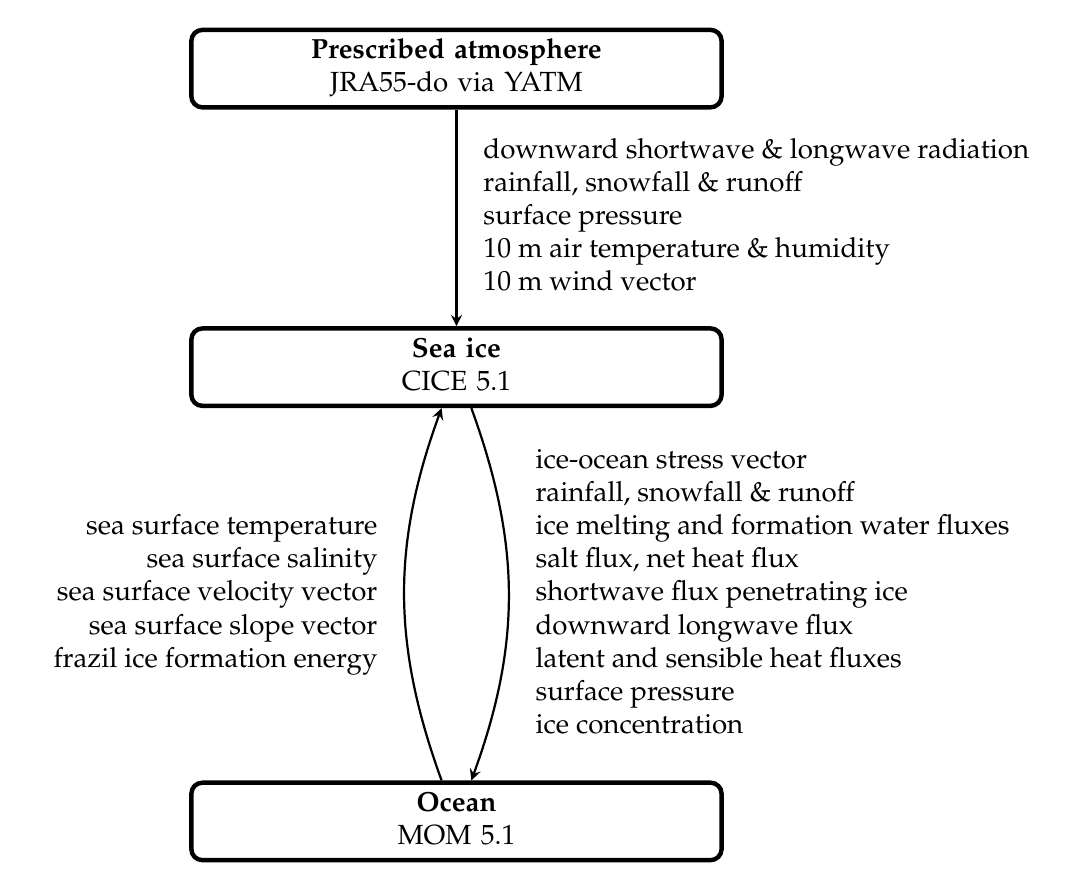
\begin{tikzpicture}[->,>=stealth,thick]
            
%             \node[state, text width=30ex] (ATM) 
             \node[state] (ATM) 
             {\begin{tabular}{c}
              \textbf{Prescribed atmosphere}\\
              JRA55-do via YATM
              \end{tabular}};
              
             \node[state, 
%              text width=30ex, 	% max text width
              below of=ATM,
              node distance=23ex,
              anchor=center] (ICE)
             {%
             \begin{tabular}{c}
              \textbf{Sea ice}\\
              CICE 5.1
             \end{tabular}
             };
             
             \node[state,
%               text width=30ex,
             below of=ICE,
              node distance=35ex,
              anchor=center
              ] (OCEAN) 
             {%
             \begin{tabular}{c}
              \textbf{Ocean}\\
              MOM 5.1
             \end{tabular}
             };
            
             \path 
             (ATM) 	edge node[anchor=south,right]
            {
            \begin{tabular}{l}
                downward shortwave \& longwave radiation\\
                rainfall, snowfall \& runoff\\
                surface pressure\\
                10 m air temperature \& humidity\\ % NB: namcouple comment is out of date - TsujinoETAL2018a state this is 10m (rather than 2m)
                10 m wind vector
            \end{tabular}
            }
                (ICE)
             (ICE)  	edge[bend left=20]                  node[anchor=left,right]
             {
            \begin{tabular}{l}
                ice-ocean stress vector\\
                rainfall, snowfall \& runoff\\
                ice melting and formation water fluxes\\
                salt flux, net heat flux\\
                shortwave flux penetrating ice\\
                downward longwave flux\\
                latent and sensible heat fluxes\\
                surface pressure\\
                ice concentration
            \end{tabular}
            }
            (OCEAN)            
            (OCEAN)  	edge[bend left=20]  node[anchor=left,left]
             {
            \begin{tabular}{r}
                sea surface temperature\\
                sea surface salinity\\
                sea surface velocity vector\\
                sea surface slope vector\\
                frazil ice formation energy
            \end{tabular}
            }
            (ICE)
            ;
        
        \end{tikzpicture}
    \end{center}
    \caption[Coupling between model components.]{
    Coupling between model components by OASIS3-MCT as specified in the namcouple file.
    Notice that MOM receives atmospheric forcing via CICE rather than directly from YATM (CICE has the same global domain as MOM).
}
    \label{F:coupling}
\end{figure}

%namcouple file list coupled fields
%
%atmosphere to ice: downward shortwave and longwave radiation, rainfall, snowfall, runoff, surface pressure, air temperature, humidity, 10m wind vector
%
%ice to atmosphere: 
%
%ice to ocean: stress vector, freshwater flux from rainfall and snowfall, runoff, salt flux, heat flux, shortwave flux penetrating ice, longwave flux, latent and sensible heat flux, surface pressure, ice concentration, ice melting and forming water fluxes
%
%ocean to ice: sea surface temperature, salinity, slope vector and velocity vector, frazil ice formation energy


\subsection{Forcing}

There are no tides but there is parameterised internal tidal mixing.

We have mass exchange of surface freshwater fluxes as in \citet{BiMarslandUotilaOFarrellFiedlerSullivanGriffiesZhouHirst2013a} \TODO{confirm}

JRA55-do v1.3 atmospheric forcing (1984-5, 1990-1 or 2003-4 repeat-year, 0.5625$^\circ$ ($\sim$55km), 3-hourly) in addition to CORE NYF (2$^\circ$ ($\sim$200\,km), 6-hourly)

JRA-55-do v1.3 forcing is supported at all three resolutions, and CORE2 forcing is supported at 1 degree resolution. 
JRA-55-do repeat-year forcing forcing (RYF) and interannual forcing (IAF) and CORE normal-year forcing (NYF) are currently supported. \FIXME{what about CORE IAF?}

\subsubsection{JRA55-do interannual and repeat-year forcing}

The ACCESS-OM2 configurations are forced with the latest JRA55-do v1.3 atmospheric reanalysis \citep{TsujinoETAL2018a} which has significantly improved bias, spatial and temporal resolution (55 km, 3-hourly), temporal extent (1958--2018), and dynamical self-consistency compared to the CORE dataset (200 km, 6-hourly, 1948--2009) used in many previous studies. We use recent calving and basal melt estimates from \citet{DepoorterBamberGriggsLenaertsLigtenbergBroekeMoholdt2013a}, which are spatially variable and somewhat larger than the uniform values in CORE \citep{TsujinoETAL2018a}. JRA55-do will also be regularly updated, allowing real-time experiments. The improved spatial resolution of wind is important for better representation of coastal polynyas \citep{StosselZhangVihma2011a, ZhangVihmaStosselUotila2015a}.
JRA55-do has higher spatial and temporal resolution and longer temporal extent than ERA-Interim (80\,km, 6-hourly, 1979--present) % https://www.ecmwf.int/en/forecasts/datasets/archive-datasets/reanalysis-datasets/era-interim
but is coarser and somewhat shorter than the upcoming ERA5 reanalysis (31\,km, 3-hourly, 1950--present): \url{https://confluence.ecmwf.int//pages/viewpage.action?pageId=74764925}.% https://www.ecmwf.int/en/forecasts/datasets/archive-datasets/reanalysis-datasets/era5


See JRA55_RYF_justification.ipynb for biases in each RYF year.

JRA55-do \citep{TsujinoETAL2018a} is a surface-atmospheric reanalysis product derived from the 55-year Japanese reanalysis (JRA55, \url{http://jra.kishou.go.jp/JRA-55/index_en.html}) and intended for driving oceans models. 
We use JRA55-do version 1.3 to drive our ice and ocean models.
The temporal coverage is from 1st January 1958 to 1st February 2018, but it is regularly updated to near present day.



\url{http://climate-cms.unsw.wikispaces.net/JRA55-do} - data in /g/data/ua8/JRA55-do/latest/
% /g/data1/rr7/JRA55 is full JRA55

JRA55-do user manual: \citet{TsujinoUrakawaNakanoSmallKimYeagerDanabasogluSuzukiBamber2018a}

Data available from \url{https://esgf-node.llnl.gov/search/input4mips/?institution_id=MRI}
and on NCI at /g/data1/ua8/JRA55-do/RYF/v1-3/*.nc

For the latest information on the dataset status and citation: \url{http://goo.gl/r8up31}.

see \url{http://amaterasu.ees.hokudai.ac.jp/~tsujino/JRA55-do-v1.3/00README_v1_3.1st}
JRA-55: \citet{KobayashiOtaHaradaEbitaMoriyaOnodaOnogiKamahoriKobayashi2015a}
JRA55-do: \citet{Tsujino2015a, Tsujino2015b, Tsujino2016a, TsujinoETAL2018a}, \citet{TsujinoUrakawaSuzukiKomuroSmallKimYeagerDanabasogluGriffies2016a},
\citet{KimSmallYeagerDanabasogluTsujinoETAL2018a}


\url{http://www.clivar.org/omdp/japan2016}

JRA55-do version 1.3 provides
3-hourly liquid and solid precipitation, downwelling surface longwave and shortwave radiation, sea level pressure, 10m wind velocity components, 10m specific humidity and 10m air temperature 
on a TL319 grid (0.5625$^\circ$ resolution), and daily river flux at 0.25$^\circ$ resolution.

\TODO{check: what do we use for glacier runoff? groundwater? evaporation? upwelling longwave radiation?}

``Runoff from Greenland and Antarctica are replaced by climatological runoff.
Greenland runoff is based on \citet{BamberBroekeEttemaLenaertsRignot2012a} and Antarctica runoff
is based on \citet{DepoorterBamberGriggsLenaertsLigtenbergBroekeMoholdt2013a}.'' (\url{http://amaterasu.ees.hokudai.ac.jp/~tsujino/JRA55-do-v1.3/00README_v1_3.1st})

The Antarctic runoff is spatially variable in JRA55-do \citep{TsujinoETAL2018a}, in contrast to CORE .

we made a start on this: \url{https://github.com/OceansAus/matm/issues/5}

should we / do we use this for runoff? \citet{SuzukiYamazakiTsujinoKomuroNakanoUrakawa2017a}

currently fresh water is input at the ice shelf edges.

cf.\ runoff (iceberg discharge scheme) used in ACCESS-CM2 - see AMOS2018 notes on Dave Bi's talk and \url{https://accessdev.nci.org.au/trac/wiki/CMIP6workshop}
--- this is discharged only at the surface.
See Siobhan's email 2018-06-04

Runoff - incl distributed iceberg melt? Ask Adele? basal melt needs to be at depth - notebook p561. We have the data but waiting on it being published. 
Veronique has regridded this - see email 2017-11-16 \citet{MerinoLeSommerDurandJourdainMadecMathiotTournadre2016a} and
\citet{DepoorterBamberGriggsLenaertsLigtenbergBroekeMoholdt2013a}
Paul: ``The Antarctic ice berg data is published and the data is publicly available here: 
\url{http://neichin.github.io/personalweb/publications/}
However, the Antarctic basal melt fluxes are not published yet and the data has not been made public.''
Also see \citet{MerinoJourdainLe-SommerGoosseMathiotDurand2018a, Donat-MagninJourdainSpenceLe-SommerGalleeDurand2017a, MathiotJenkinsHarrisMadec2017a,HammondJones2016a, StosselNotzHaumannHaakJungclausMikolajewicz2015a}

Runoff - what range of depths is used? Top 4 levels??


discuss choice of year for RYF --- will use 1984-5 for high-res runs -- refer to Kial's paper

These 12-month periods were identified as particularly "neutral":
1 May 1984 - 30 April 1985,
1 May 1990 - 30 April 1991,
1 May 2003 - 29 April 2004 (we keep 29 Feb 2004 and ditch 30 April 2004 so as to keep 365 days per year).
We have run ocean-sea ice spinups forced by all three JRA55-do v1.3 repeat years at 1$^\circ$ but we are concentrating on 1984-5 for the 1/10$^\circ$ spinup as it has less of the warming signal and also gives us more of the JRA55 dataset for subsequent interannual runs.

Kial's email 2018-03-05:
\begin{quote}
-1st of January is in the peak of the northern winter and southern summer, meaning the variability in forcing fields (ie. weather) is quite high. This is a problem for surface buoyancy fluxes in the north Atlantic and Labrador \& Nordic Sea regions, where NADW formation is notoriously sensitive to changes in surface forcing. The day of the year with lowest variability (least weather) is going to be closer to the equinoxes, and in JRA55 DO it turns out to be 1 May. 

-The three candidate years have been selected as the 12-month periods with climate indices closest to neutral. The climate indices of interest are the SOI, SAM and NAO. Removing the criteria that a 12-month period follows the calendar year allows us to find "years" that are closer to climatologically neutral.

-Having the jump at 1 May allows us to run the model harder. The model tends to fall over at 1 Jan if the jump is there, meaning we have to back off the timestep and nurse it through. Having the jump at 1 May does not require any such nursing. Currently we are running the ACCESS-OM2 1$^\circ$ with 5400 sec timesteps from initialization and getting through ~90 years per day.
\end{quote}
\TODO{plots of anomalies from climatology for the time-mean (or seasonal-mean) RYF forcing fields}


see \url{https://github.com/OceansAus/access-om2/issues/52} and \url{http://www.earthsystemmodeling.org/esmf_releases/last_built/ESMF_refdoc/node3.html#SECTION03020000000000000000}


\subsubsection{CORE-NYF}
\url{http://www.clivar.org/clivar-panels/omdp/core-2}
2$^\circ$, 6-hourly

\subsubsection{Restoring}

The only restoring we apply is to surface salinity.
This is restored to interpolated \TODO{state interpolation method --- Smoothing at 0.1deg to deal with spurious discontinuities and noise in WOA13v2: \url{https://github.com/OceansAus/access-om2/issues/103}} World Ocean Atlas 2013 v2 monthly climatology (\url{https://www.nodc.noaa.gov/OC5/woa13/}); the interpolated salinity file is salt_sfc_restore.nc. % ncdump -h salt_sfc_restore.nc gives: This salinity distribution is based on WOA13v2 where the land values are filled in with a conjugate gradient method. It is a simple average of land-filled salinity data at the depth of 0 and 10 meters.
The restoring timescale is set by \mom{salt_restore_tscale}; we use 10 days at 0.1$^\circ$ and 60 days for the coarser resolutions.
The ``piston velocity`` (surface vertical grid spacing divided by restoring timescale) is more physically relevant than the restoring timescale.
This is 0.11\,m/day at 0.1$^\circ$ and 0.17\,m/day for the coarser models due to the differing vertical resolution (see table~\ref{T:vgrid}).
For comparison, 15\,m/300\,days (i.e.\ 0.05\,m/day) is GFDL's standard piston velocity (Griffies, 12 April 2018), so we are restoring more strongly than GFDL.

We also limit restoring flux (\mom{max_delta_salinity_restore} = 0.5\,psu).
We apply salinity restoring via a salt flux (\mom{use_waterflux} =  true, \mom{salt_restore_as_salt_flux} = true) and restore everywhere, including under ice (\mom{salt_restore_under_ice} = true).
A spatially constant offset is added to the salt restoring to ensure that the net salt restoring flux is zero for each timestep (\mom{zero_net_salt_restore} = true).
\TODO{discuss these - Normalise P+R-E? }
\mom{zero_net_water_coupler} = true
\mom{zero_net_water_restore} = true
These choices are typical of CORE-II models \citep[][table~2]{DanabasogluYeagerBaileyBehrensBentsenBiBiastochBoningBozec2014a}.

See \citet[][section~2.3]{GriffiesETAL2016a} and \citet[][Appendix~C]{DanabasogluYeagerBaileyBehrensBentsenBiBiastochBoningBozec2014a}.
Sensitivity to restoring: \citet{BehrensBiastochBoning2013a}.

2nd order conservative interpolation:
\citet{KritsikisAechtnerMeurdesoifDubos2017a}

\subsubsection{Sea ice formation salt flux limiter}
The model sea ice has a fixed bulk salinity (we use the default \mom{ice_salt_concentration} = 0.005 kg salt / kg ice). 
This salt is obtained from the seawater when sea ice is formed, and we found this could drive ocean salinity below zero in regions fresher than \mom{ice_salt_concentration}, for example during the spring melt in the shallow Siberian gulfs that are resolved in the 0.1$^\circ$ model bathymetry.
This problem was resolved by setting the local ocean-ice salt flux to zero in regions where the seawater salinity is less than \mom{ocean_ice_salt_limit} = 0.006 kg salt / kg ice.
Since we use \mom{zero_net_salt_restore} = true, in these regions the sea ice salt is instead obtained from the global surface ocean at large.
Over a sea ice formation and melt cycle this produces a small unphysical transport of salt from the global surface ocean to regions where such sea ice melts.
Sea ice formed in regions saltier than \mom{ocean_ice_salt_limit} obtains its salt locally as usual.
\TODO{get Russ to check this} 
\url{https://github.com/mom-ocean/MOM5/commit/2d76b70ca66173f8dfcfdb0597c9b148ef4a7510}
This limiter is only applied in the 0.1$^\circ$ model.

\subsubsection{Bulk formulas used}
These are specified in the AUSCOM ocean drivers.

see \url{https://github.com/OceansAus/cice5/blob/master/source/ice_atmo.F90}, 
\url{https://github.com/OceansAus/cice5/blob/master/source/ice_forcing.F90},
\url{https://github.com/OceansAus/cice5/blob/master/drivers/auscom/surface_flux_mod.F90}

We use \citet{LargeYeager2004a} turbulent flux bulk formulas (\cice{ncar_ocean_flux}=true, \cice{ncar_ocean_flux_orig}=false), for the air-ocean drag coefficient, evaporative transfer coefficient and sensible heat transfer coefficient \citep[eq.\ 6--10 in ][]{LargeYeager2004a}. 
This is implemented in \url{https://github.com/OceansAus/cice5/blob/master/drivers/auscom/surface_flux_mod.F90#L896}. 
The calculation uses the air-ocean velocity difference with an additional component to account for gustiness (the gust component is derived from \FIXME{what?} and is not modified: \cice{alt_gustiness}, \cice{gust_const}, \cice{gust_min}).
Note that the implementation differs from \citet{LargeYeager2004a} in having a \SI{0.5}{m.s^{-1}} floor for the 10\,m relative windspeed, a ceiling of 10 for the absolute value of the stability parameter $\zeta$, and a floor of 1 for the parameter $X=(1-16\zeta)^\frac{1}{4}$ (though the last of these should have no effect). 
We used \param{\href{https://github.com/OceansAus/cice5/search?q=n_itts}{n_itts}}=2 Monin-Obukhov iterations, which \citet{LargeYeager2004a} state is appropriate for over the ocean, but less than their suggested value of 5 for over sea ice. \FIXME{or is this only applied over the ocean?}

\citet{LargeYeager2009a}

- relative or absolute wind? \citet{AbelBoningGreatbatchHewittRoberts2017a}
looks like we use relative wind: \url{https://github.com/OceansAus/cice5/blob/master/drivers/auscom/surface_flux_mod.F90#L548} - relative to ice as well as ocean? what happens when ice coverage is not 0\% or 100\%?
See \citet[][, section~3.4.3]{TsujinoETAL2018a}: raw JRA55 winds have been adjusted in JRA55-do to agree with scatterometer and radiometer winds, which are relative to the ocean current. 
So subtracting the ocean surface current may be unnecessary.
\citet{Tsujino2018a} recommend adding the climatological surface current distributed with the forcing dataset to better approximate the absolute wind.
see \citet{WuZhaiWang2017a} and  \url{https://arccss.slack.com/archives/C6PP0GU9Y/p1511825314000106?thread_ts=1511802000.000465&cid=C6PP0GU9Y}
and \url{https://jra55-do.slack.com/archives/C7LEZT4KY/p1511963905000047} and \url{https://github.com/OceansAus/access-om2/issues/79}

\TODO{should bulk formulas match what was used in JRA55-do?} do we need something like ncar_ocean_fluxes but for JRA-55? \url{https://github.com/OceansAus/cice5/blob/master/drivers/auscom/surface_flux_mod.F90#L820} NB: \citet{TsujinoETAL2018a} use formulas \citet{Gill82a} and recommend using these rather than \citet{LargeYeager2004a, LargeYeager2009a}


see \citet{RobertsCraigMaslowskiOsinskiDuvivierHughesNijssenCassanoBrunke2015a} appendix A  - RASM uses nonzero ice velocity for stress calculation

cf.\ appendix C of \citet{GriffiesBiastochBoningBryanDanabasogluChassignetEnglandGerdesHaak2009a}.

\subsubsection{YATM}
\CONTRIBUTORS{Nic Hannah}

See \url{http://cosima.org.au/wp-content/uploads/2018/06/COSIMA2018-Hannah.pdf}

YATM parameters for the three model resolutions are tabulated in Appendix~\ref{S:yatm-namelist}.

SCRIP regridding for OASIS3-MCT does not scale to 0.1$^\circ$, so instead we use ESMF\_RegridWeightGen from ESMF (\url{https://www.earthsystemcog.org/projects/esmf/}); this also allows smoother conservative interpolation, which is needed for the 0.25$^\circ$ and 0.1$^\circ$ configurations as they are finer than the forcing datasets.
The regridding method is documented at \url{https://github.com/OceansAus/access-om2/wiki/Creating-Remapping-Weights}.

YATM remaps runoff in real time using an algorithm based on KDTREE2 (\url{https://github.com/jmhodges/kdtree2}), with spatially variable conservative flux limiting (values are set by \yatm{runoff_caps} in units of kg\,m$^{-2}$\,s$^{-1}$; $i$-index start and end regions are set by \yatm{runoff_caps_is} and \yatm{runoff_caps_ie}, and $j$-index start and end regions are set by \yatm{runoff_caps_js} and \yatm{runoff_caps_je}).
\TODO{Tabulate / plot runoff caps in all models}
\FIXME{what runoff caps are applied at 1deg and 0.25deg?}

\subsection{Initial conditions and spinup}
Initial condition is from World Ocean Atlas 2013 v2 \url{https://www.nodc.noaa.gov/OC5/woa13/}.

What's the sea ice initial condition? 3m at pole, dropping off with latitude equatorward?? - Siobhan - 
parameter ice\_ic = 'default' 
'default'  = latitude and sst dependent
\url{https://github.com/OceansAus/cice5/blob/5583ce54fd8822c1b8aef0549090167ca5f36d10/source/ice_init.F90#L23}
sets up ice where SST is cold, max 3m thick...?
\url{https://github.com/OceansAus/cice5/blob/5583ce54fd8822c1b8aef0549090167ca5f36d10/source/ice_init.F90#L1538}

\subsection{Model computational details and performance}
\CONTRIBUTORS{Marshall}

\TODO{cannibalise NCMAS application}

Discuss timestep choices at each resolution.

\citet{CraigMickelsonHunkeBailey2014a}?

old MOM benchmarks: \citet{Schmidt2007a}?

cf. \ MOM-SIS-01: 50--60kSU/day? - check with Andy

1/10$^\circ$: 1200 PUs for CICE + 4358 PUs for MOM + 1 for YATM \TODO{update}

Typical walltimes: \TODO{check/update these. how many z levels?}
\begin{itemize}
\item ACCESS-OM: $\sim 16$min/yr on 252 PEs, dt=5400s
\item ACCESS-OM-025: $\sim 60$min/yr on 1960 PEs, dt=1800s
\item ACCESS-OM-01: $\sim 18$hr/yr on 6359 PEs, dt=540s
\end{itemize}


\TODO{cf. Matt Chamberlain's 2016 talk: global MOM-SIS at 1/10$^\circ$ and 50 levels, 960 CPUs (50x23 layout, 200 masked), dt=720s, month $\sim$100min: \url{http://cosima.org.au/wp-content/uploads/2016/06/ofam_global.mac_.pdf} --- this is as fast as ACCESS-OM2-01 but about 6x cheaper!}

see layout in ocean/input.nml: plot MOM tiling, showing dry tiles and bathymetry for each resolution

see BLCKX, BLXKY in cice5/bld/config.nci.auscom.3600x2700 etc - plot CICE tiling, showing idle tiles for each resolution


MOM barotropic/baroclinic split, timesteps


mom tile layout: /short/v45/raf599/masking/procno_045x036_5000.nc

\subsection{Comparison with similar models}
Namelists of MOM-based models are compared in Appendix~\ref{S:namelist-model-comparisons}.


\begin{table}%[htdp]
\caption{ACCESS-OM2 updates and extends ACCESS-OM and OFAM3.}
\begin{center}
\begin{tabular}{|c|c|c|c|}
\hline
& \textbf{ACCESS-OM} & \textbf{OFAM3} & \textbf{ACCESS-OM2}\\
\hline
Ocean & MOM~4.1 & MOM~4.1 & MOM~5.1\\
Sea ice & CICE~4.1 & --- & CICE~5.1\\
%Atmosphere & MATM & --- & YATM\\
%Forcing & & JRA55-do (XX$^\circ$, 6hr)&\\\
Coupler & OASIS~3.25 & --- & OASIS 3-MCT\\
%Interpolation & SCRIP & --- & ESMF (at all resolutions??)\\
Grid & global tripolar, $z^*$ & 75$^\circ$S--75$^\circ$N only, $z^*$ & global tripolar, $z^*$\\
Resolution & 
1$^\circ$, 360$\times$300$\times$50 & 
\parbox[][][c]{22ex}{%
0.1$^\circ$, 3600$\times$1500$\times$51, $\Delta z$=5 -- 1000m 
} &
\parbox[][][c]{22ex}{%
1$^\circ$, 360$\times$300$\times\\$(50, 75 or 100 levels)\\
or\\0.25$^\circ$,~1440$\times$1080$\times$50,\\$\Delta z=10.1$ -- 210m\\
or\\0.1$^\circ$, 3600$\times$2700$\times$75, $\Delta z$=1.1 -- 198m\\[-1ex]}\\
%Resolution & 1$^\circ$, 360$\times$300$\times$50 & \parbox[][][c]{20ex}{0.1$^\circ$ near Aust, up to 2$^\circ$ elsewhere, 1191$\times$968$\times$47} & \parbox[][][c]{20ex}{1$^\circ$, 360$\times$300$\times\\$(50, 75 or 100 levels)\\or\\0.25$^\circ$,~1440$\times$1080$\times$50\\or\\0.1$^\circ$, 3600$\times$2700$\times$75}\\
%Top layer thickness & ? & 5\,m 
%\rowcolor{white}& & &                                                  0.25$^\circ$, 1440$\times$1080$\times$50\\
%& & &                                                  0.1$^\circ$, 3600$\times$2700$\times$75\\
%Initial condition & WOA~2005 & global CARS & WOA~2013~v2\\
%\vspace{2ex}
\hline
\end{tabular}
\end{center}
\label{T:access-om-ofam3-access-om2}
\end{table}

\subsubsection{GFDL CM2, CM2.5, CM2.6}
cf. CM2-1deg CM2.5 CM2.6 (they were MOM v5) and discuss resolving eddies: \citet{GriffiesWintonAndersonBensonDelworthDufourDunneGoddardMorrison2015a}
\citet{DelworthRosatiAndersonAdcroftBalajiBensonDixonGriffiesLee2012a}
\citet{DunneJohnAdcroftGriffiesHallbergShevliakovaStoufferCookeDunne2012a}
\citet{Griffies2015a}

cf.\ CORE \citep{GriffiesBiastochBoningBryanDanabasogluChassignetEnglandGerdesHaak2009a}, CORE-II \citep{DanabasogluYeagerBaileyBehrensBentsenBiBiastochBoningBozec2014a}

minimum depth = 40m ?

\subsubsection{ACCESS, ACCESS-CM2, ACCESS-ESM}
See \url{https://accessdev.nci.org.au/trac/wiki/CMIP6workshop}
There's an ACCESS-CM2 report available - ask Arnold Sullivan.
And data is available on NCI to members of p66 and NCI access groups

ACCESS-OM2 uses the same MOM, CICE and OASIS versions as ACCESS-CM2 (1$^\circ$)

cf. ACCESS \citet{BiDixMarslandOFarrellRashidUotilaHirstKowalczykGolebiewski2013a, BiMarslandUotilaOFarrellFiedlerSullivanGriffiesZhouHirst2013a, DixVohralikBiRashidMarslandOFarrellUotilaHirstKowalczyk2013a}

\citet{BiMarslandUotilaOFarrellFiedlerSullivanGriffiesZhouHirst2013a}

cf. ACCESS-CM2 \citet{BiYanSullivan2016a}, \url{http://cosima.org.au/wp-content/uploads/2016/06/BI-COSIMA-Hobart-20160526.ppt.pdf} - Uses same MOM, CICE and OASIS versions as ACCESS-CM2

cf. ACCESS-ESM \url{https://www.google.com.au/url?sa=t&rct=j&q=&esrc=s&source=web&cd=2&ved=0ahUKEwjvjsmH0rjZAhWEnpQKHb7VC-EQFgg0MAE&url=https%3A%2F%2Faccessdev.nci.org.au%2Ftrac%2Fraw-attachment%2Fwiki%2FScienceDay%2Fziehn_access_esm1.pdf&usg=AOvVaw1bYwLzey6vpy7g6v7W0aF0}

\subsubsection{Antarctic Tidal Ocean Model}
The Antarctic Tidal Ocean Model is a regional circum-Antarctic model based on ROMS. Key differences from ACCESS-OM2-01 include: circulation within cavities under ice shelves, tidal forcing, shelf melting and  higher resolution (2km, 31 sigma layers). There is no sea ice model component.
% see /Users/andy/Documents/COSIMA/Antarctic Tidal Ocean Model

\subsubsection{OFAM3}
cf. OFAM3 namelists - see Matt Chamberlain's email 28 May 2018

cf. oceanMAPS3.0  \url{http://cosima.org.au/wp-content/uploads/2016/06/Brassington_Ocean_modelling_and_forecasting_v3.pptx.pdf} % /Users/andy/Documents/COSIMA/COSIMA workshop 26-27 May 2016/Gary Brassington (BoM) Brassington_Ocean_modelling_and_forecasting_v3.pptx.pdf

The vertical resolution has also been improved relative to OFAM3 \citep{OkeETAL2013a}. 
The resolution is finer tham OFAM3 at all depths other than 100--260\,m, particularly at the surface and in the deep ocean, with 75 levels ranging from 1.1m thick at the surface to 198m thick at 5808m (compared to 51 levels ranging from 5m to 1000m thick currently in OFAM3/Bluelink). 
Of particular relevance for coastal studies is the improved vertical resolution in the upper ocean, with 31 levels in the top 200m and a minimum water depth of 10m (rather than 24 levels and a minimum depth of 15m for OFAM3), providing better resolution of shelf processes and a closer match to coastlines. 
Vertical spacing is optimised for resolving baroclinic modes, considerably reducing the error in their representation compared to the 51-level OFAM3 grid \citep[][ table~1]{StewartHoggGriffiesHeerdegenWardSpenceEngland2017a}.

\citet{FengZhangOkeMonselesanChamberlainMatearSchiller2016a}

\subsubsection{MOM-SIS-01}
cf. MOM-SIS-01 \citet{SpenceHolmesHoggGriffiesStewartEngland2017a} - forced by 2$^\circ$ CORE NYF - 75 levels; ACCESS-OM2-01 has newer bathy, CICE, JRA55-do, and probably different vertical grid

ACCESS-OM2-01 has newer forcing and bathymetry, and a different sea ice model than MOM-SIS-01 \cite{SpenceHolmesHoggGriffiesStewartEngland2017a}.

\subsubsection{UKMO GO6, GO7}
cf UKMO GO6, GO7 \citet{StorkeyBlakerMathiotMegannAksenovBlockleyCalvertGrahamHewitt2018a} - based on NEMO.

GO7 has cavities under the ice shelves, whereas GO6 is similar to ACCESS-OM2-x in having no cavities and fresh water input at the ice shelf edges.

\subsubsection{RASM?}
\citet{CassanoDuVivierRobertsHughesSeefeldtBrunkeCraigFiselGutowski2017a,HammanNijssenRobertsCraigMaslowskiOsinski2017a,JinDealMaslowskiMatraiRobertsOsinskiLeeFrantsElliott2018a,RobertsHunkeAllardBaileyCraigLemieuxTurner2018a}, \url{http://www.oc.nps.edu/NAME/RASM_overview.pdf}

Key RASM differences from ACCESS-OM2-01:
\begin{itemize}
\item ndte=600 (cf 120)
\item highfreq=true
\item differing pond parameters hs0 and rfracmax
\item lots of differences in shortwave\_nml
\item differing thermo parameters chio, dSdt_slow_mode
\end{itemize}

RASM is 1/12$^\circ$ but on a rotated-pole grid so the Arctic resolution is $\sim$9\,km \citep{RobertsCraigMaslowskiOsinskiDuvivierHughesNijssenCassanoBrunke2015a}, considerably coarser than ACCESS-OM2-01 (table~\ref{T:hgrid}).

\section{Model evaluation}
 \CONTRIBUTORS{Andy Hogg to coordinate}

Data from all experiments are stored on NCI in \texttt{/g/data3/hh5/tmp/cosima} and can be accessed and analysed via the COSIMA Cookbook (\url{https://github.com/OceansAus/cosima-cookbook}).
Table~\ref{T:exptdata} specifies the subset of these experiments used for the comparisons in this section.
Data are also publicly available at \url{https://doi.org/10.4225/41/5a2dc8543105a} and \url{https://researchdata.ands.org.au/cosima-model-output-collection/993052}.

\begin{table}[tbp]
% update this with
%      python figures/exptdata.py --latex >| figures/exptdata.tex
% or
%      cd namelists; python make_nml_tables.py

\begin{tabularx}{\linewidth}{lXp{0.4\linewidth}}
\hline
\textbf{Configuration} & \textbf{Experiment} & \textbf{Path to output data on NCI} \\
\hline

ACCESS-OM2 & 1deg_jra55v13_iaf_spinup1_A & \texttt{\slash g\slash data3\slash hh5\slash tmp\slash cosima\slash access-om2\slash 1deg_jra55v13_iaf_spinup1_A}\\
ACCESS-OM2-025 & 025deg_jra55v13_iaf_gmredi & \texttt{\slash g\slash data3\slash hh5\slash tmp\slash cosima\slash access-om2-025\slash 025deg_jra55v13_iaf_gmredi}\\
ACCESS-OM2-01 & 01deg_jra55v13_iaf & \texttt{\slash g\slash data3\slash hh5\slash tmp\slash cosima\slash access-om2-01\slash 01deg_jra55v13_iaf}\\

\hline
\hline
\end{tabularx}
 
%
\begin{tabularx}{\linewidth}{lXp{0.4\linewidth}}
\hline
\textbf{Configuration} & \textbf{Experiment} & \textbf{Path to output data on NCI} \\
\hline

ACCESS-OM2 & 1deg_jra55v13_iaf_spinup1_A & \texttt{\slash g\slash data3\slash hh5\slash tmp\slash cosima\slash access-om2\slash 1deg_jra55v13_iaf_spinup1_A}\\
ACCESS-OM2-025 & 025deg_jra55v13_iaf_gmredi & \texttt{\slash g\slash data3\slash hh5\slash tmp\slash cosima\slash access-om2-025\slash 025deg_jra55v13_iaf_gmredi}\\
ACCESS-OM2-01 & 01deg_jra55v13_iaf & \texttt{\slash g\slash data3\slash hh5\slash tmp\slash cosima\slash access-om2-01\slash 01deg_jra55v13_iaf}\\

\hline
\hline
\end{tabularx}
 % use exptdata.py to automatically generate up-to-date table from latest definitions
\caption{The specific experiments used for the figures in this document.}\label{T:exptdata}
\end{table}

resolution dependence: \citet{KirtmanETAL2012a}

use obs dataset and methods from CLIVAR Repository for Evaluating Ocean Simulations? \url{http://www.clivar.org/clivar-panels/omdp/reos}
 
 cf Ocean Modelling CORE-II Special Issue (Virtual) \url{http://www.sciencedirect.com/science/journal/14635003/vsi/10PSR6J3BV4}

OMIP - \citet{GriffiesETAL2016a} - does BOM/CSIRO already have code to do this for CMIP6? ask Marsland

cf \citet{OkeETAL2013a} - reproduce some of these obs comparisons

cf \url{http://www.cesm.ucar.edu/working_groups/Ocean/metrics.html}?

cf esmvaltool \url{https://www.esmvaltool.org/}?

See Fanghua's observation comparison notebooks (should be on github) and also her presentation from 2018-01-25
and \url{https://github.com/FanghuaWu/cosima-cookbook/tree/master/notebooks}

maps of Smagorinsky biharmonic lateral viscosity? what is the viscous WBC width this implies?
- note that lateral visc is increased near western boundary, even in 0.1$^\circ$ model:  This is set by \mom{ncar_boundary_scaling} in `MOM5/src/mom5/ocean_param/lateral/ocean_bihgen_friction.F90`

see HighResMIP \citep{HaarsmaETAL2016a}

cf.\ \url{http://www.globcurrent.org}?

\subsection{Barotropic streamfunction}
late separation of Kuroshio (fig~\ref{F:Kuroshiotransport}) - cf. \citet{ColindeVerdiereOllitrault2016a}.
Problem seems to be due to WSC anomaly in RYF8485 - see Kial's emails 16 May 2018

\begin{figure}[htp]
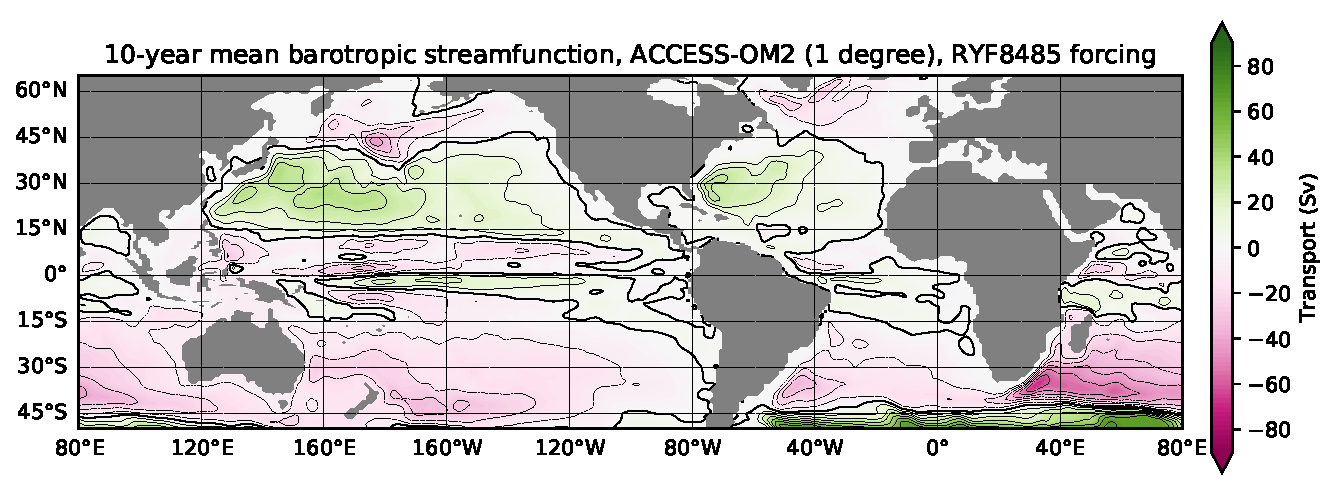
\includegraphics[width=\textwidth]{figures/BarotropicStreamfunction/gyre_transport_1deg.png}\\
\includegraphics[width=\textwidth]{figures/BarotropicStreamfunction/gyre_transport_025deg.png}\\
\includegraphics[width=\textwidth]{figures/BarotropicStreamfunction/gyre_transport_01deg.png}
\caption{Global barotropic streamfunction for ACCESS-OM2 simulations.}
\label{F:gyretransport}
\end{figure}

\begin{figure}[htp]
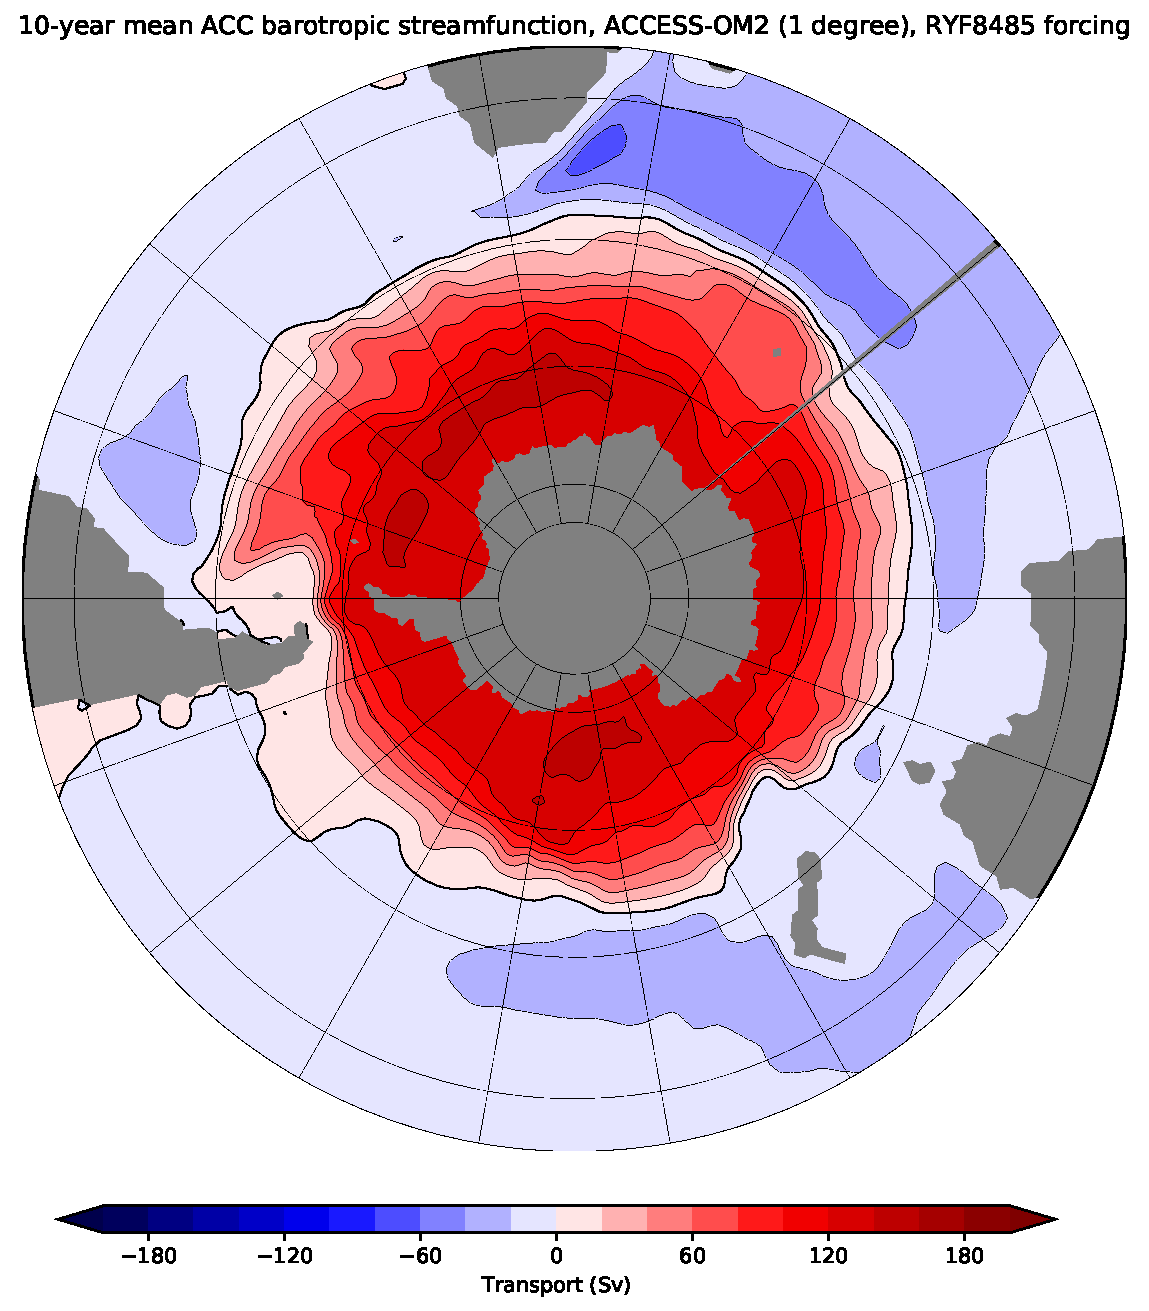
\includegraphics[width=.32\textwidth]{figures/BarotropicStreamfunction/ACC_transport_1deg.png}\hfill
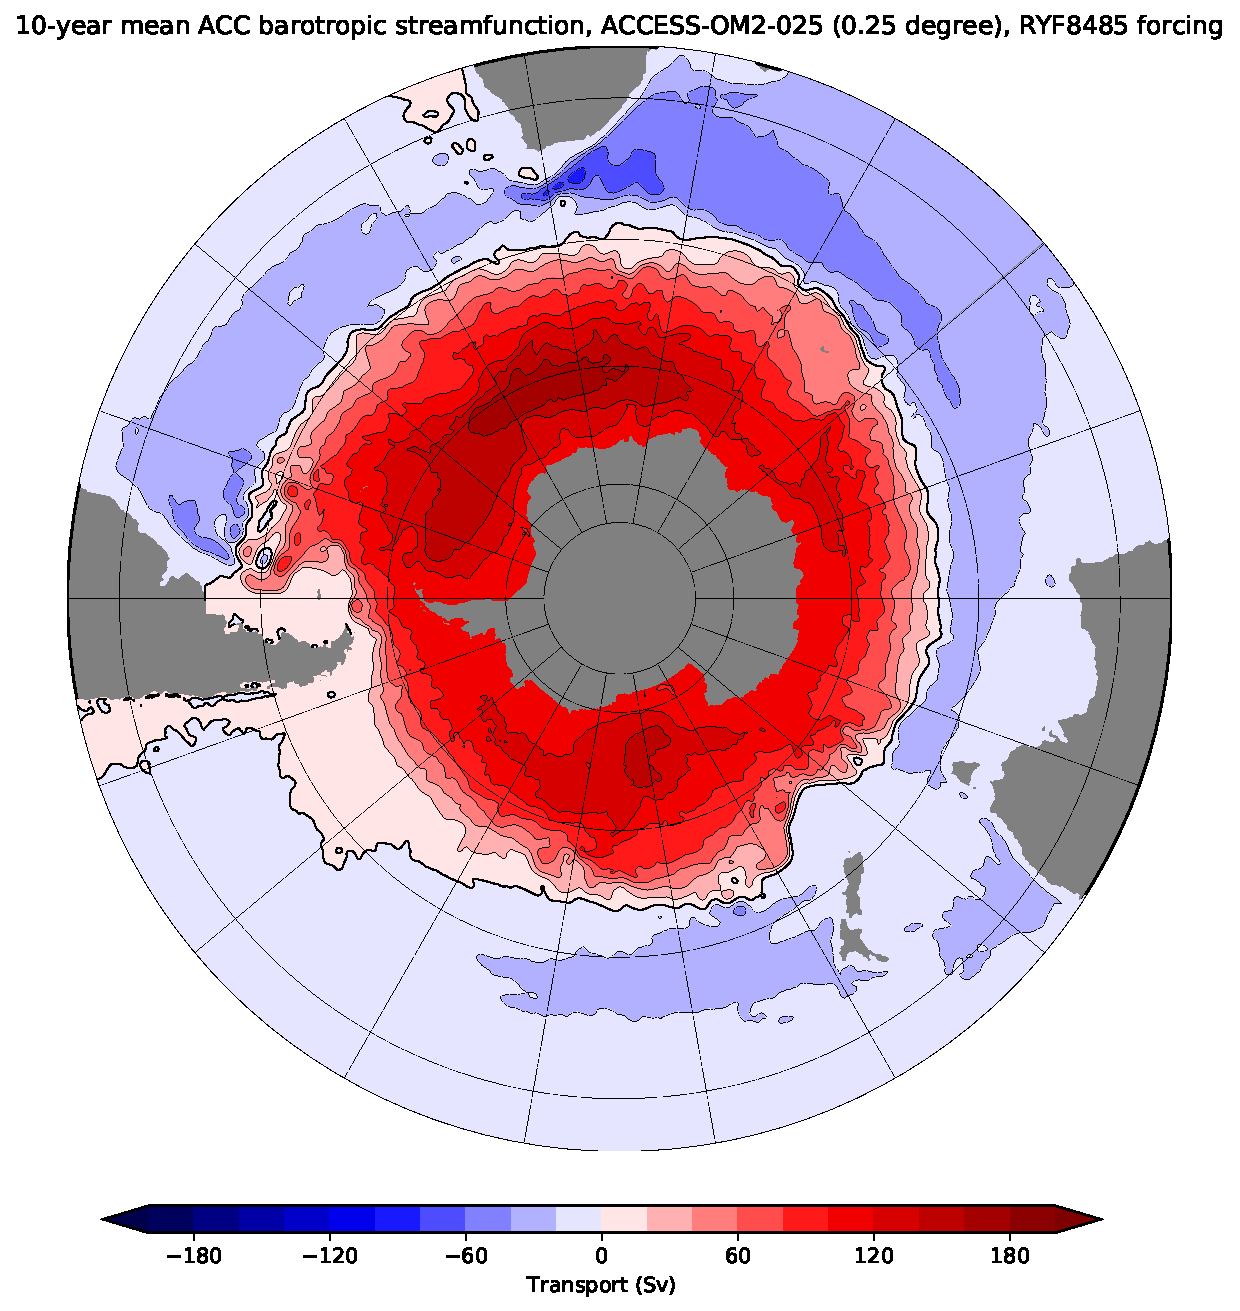
\includegraphics[width=.32\textwidth]{figures/BarotropicStreamfunction/ACC_transport_025deg.png}\hfill
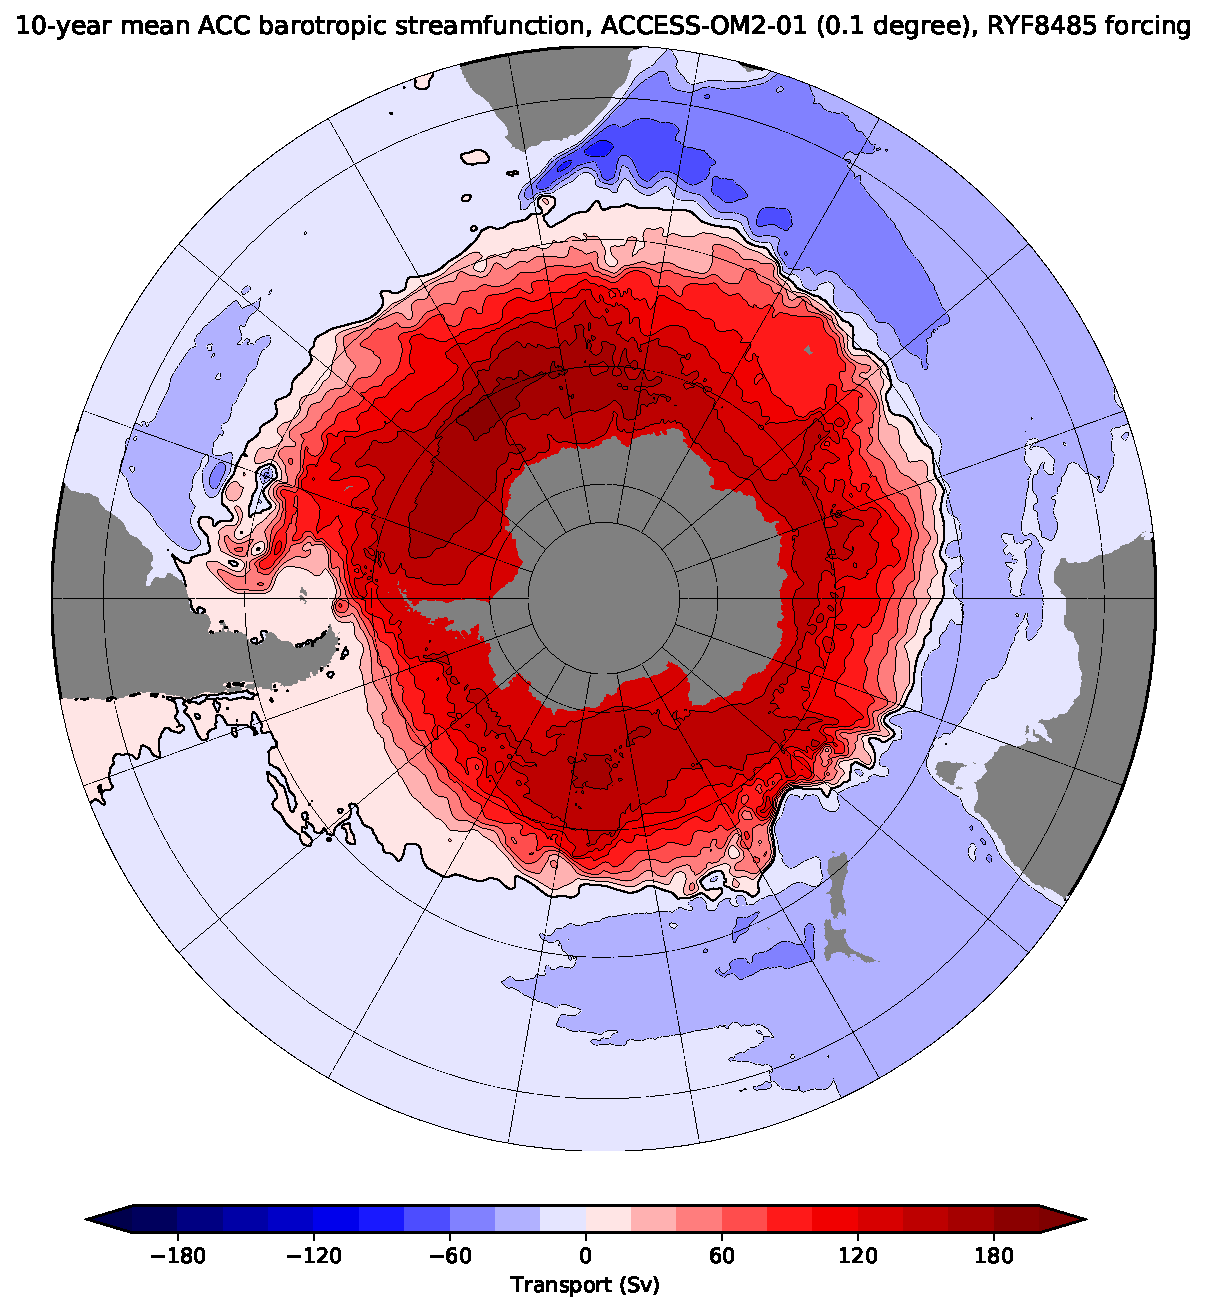
\includegraphics[width=.32\textwidth]{figures/BarotropicStreamfunction/ACC_transport_01deg.png}
\caption{Antarctic Circumpolar Current barotropic streamfunction for ACCESS-OM2 simulations. \TODO{Compare with \citet{ColindeVerdiereOllitrault2016a} figure 9:} \url{https://journals.ametsoc.org/na101/home/literatum/publisher/ams/journals/content/phoc/2016/15200485-46.1/jpo-d-15-0046.1/20160222/images/large/jpo-d-15-0046.1-f9.jpeg}}
\label{F:ACCtransport}
\end{figure}

\begin{figure}[htp]
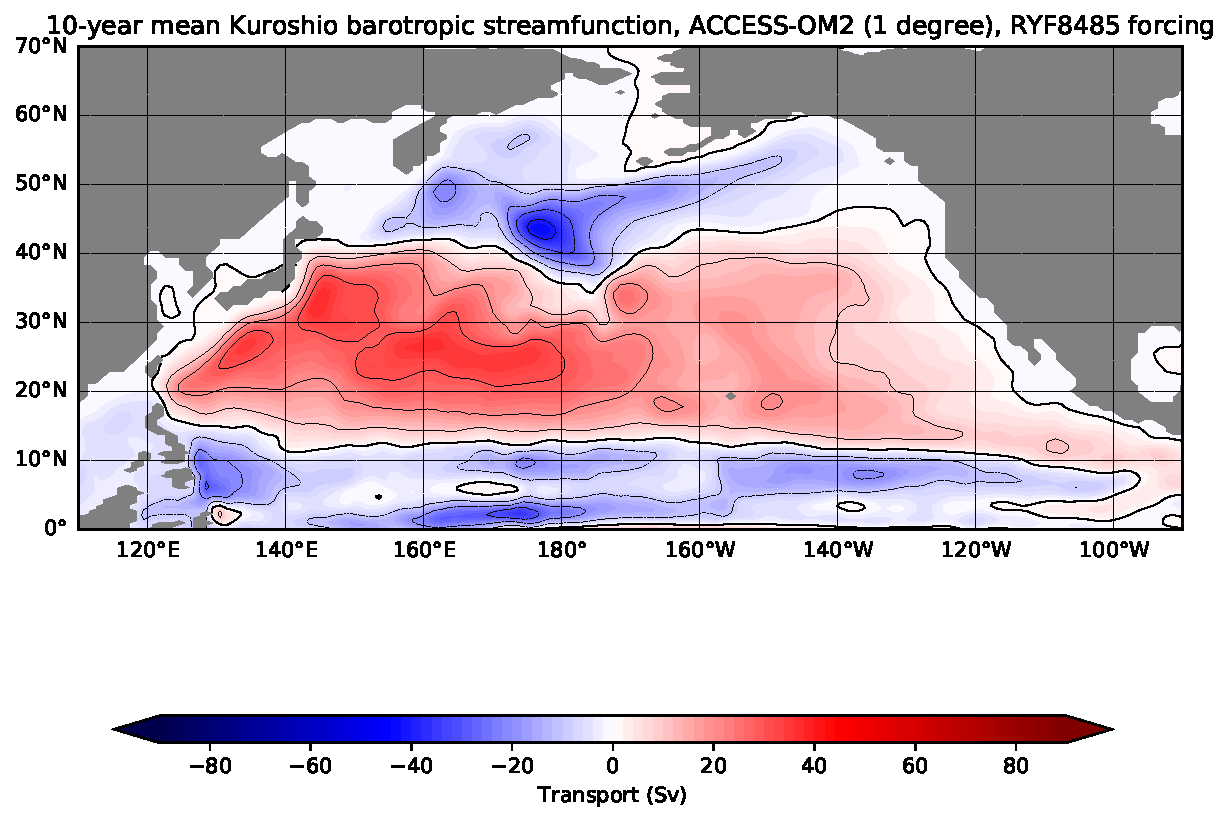
\includegraphics[width=.32\textwidth]{figures/BarotropicStreamfunction/Kuroshio_transport_1deg.png}\hfill
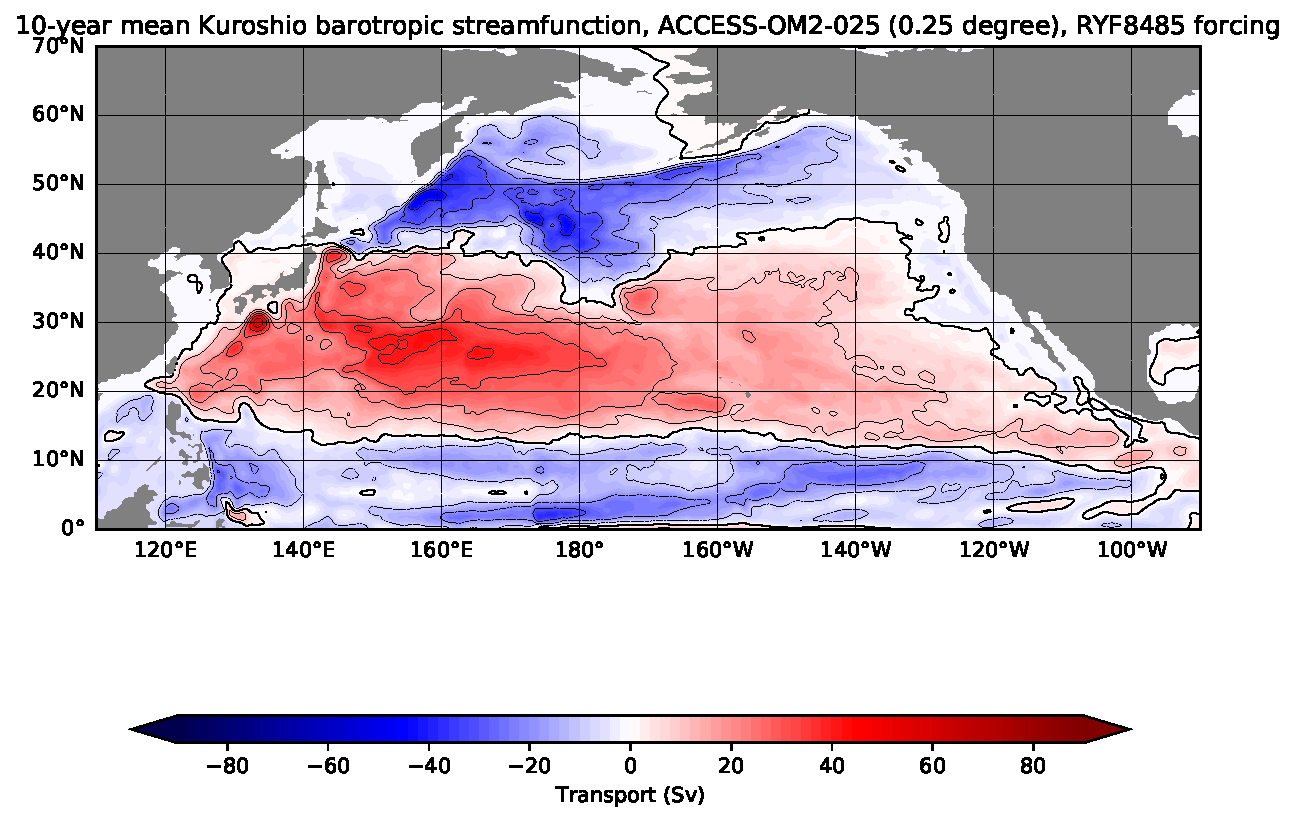
\includegraphics[width=.32\textwidth]{figures/BarotropicStreamfunction/Kuroshio_transport_025deg.png}\hfill
\includegraphics[width=.32\textwidth]{figures/BarotropicStreamfunction/Kuroshio_transport_01deg.png}
\caption{Kuroshio barotropic streamfunction for ACCESS-OM2 simulations. \TODO{Compare with \citet{ColindeVerdiereOllitrault2016a} figure 7:} \url{https://journals.ametsoc.org/na101/home/literatum/publisher/ams/journals/content/phoc/2016/15200485-46.1/jpo-d-15-0046.1/20160222/images/large/jpo-d-15-0046.1-f7.jpeg}}
\label{F:Kuroshiotransport}
\end{figure}

\begin{figure}[htp]
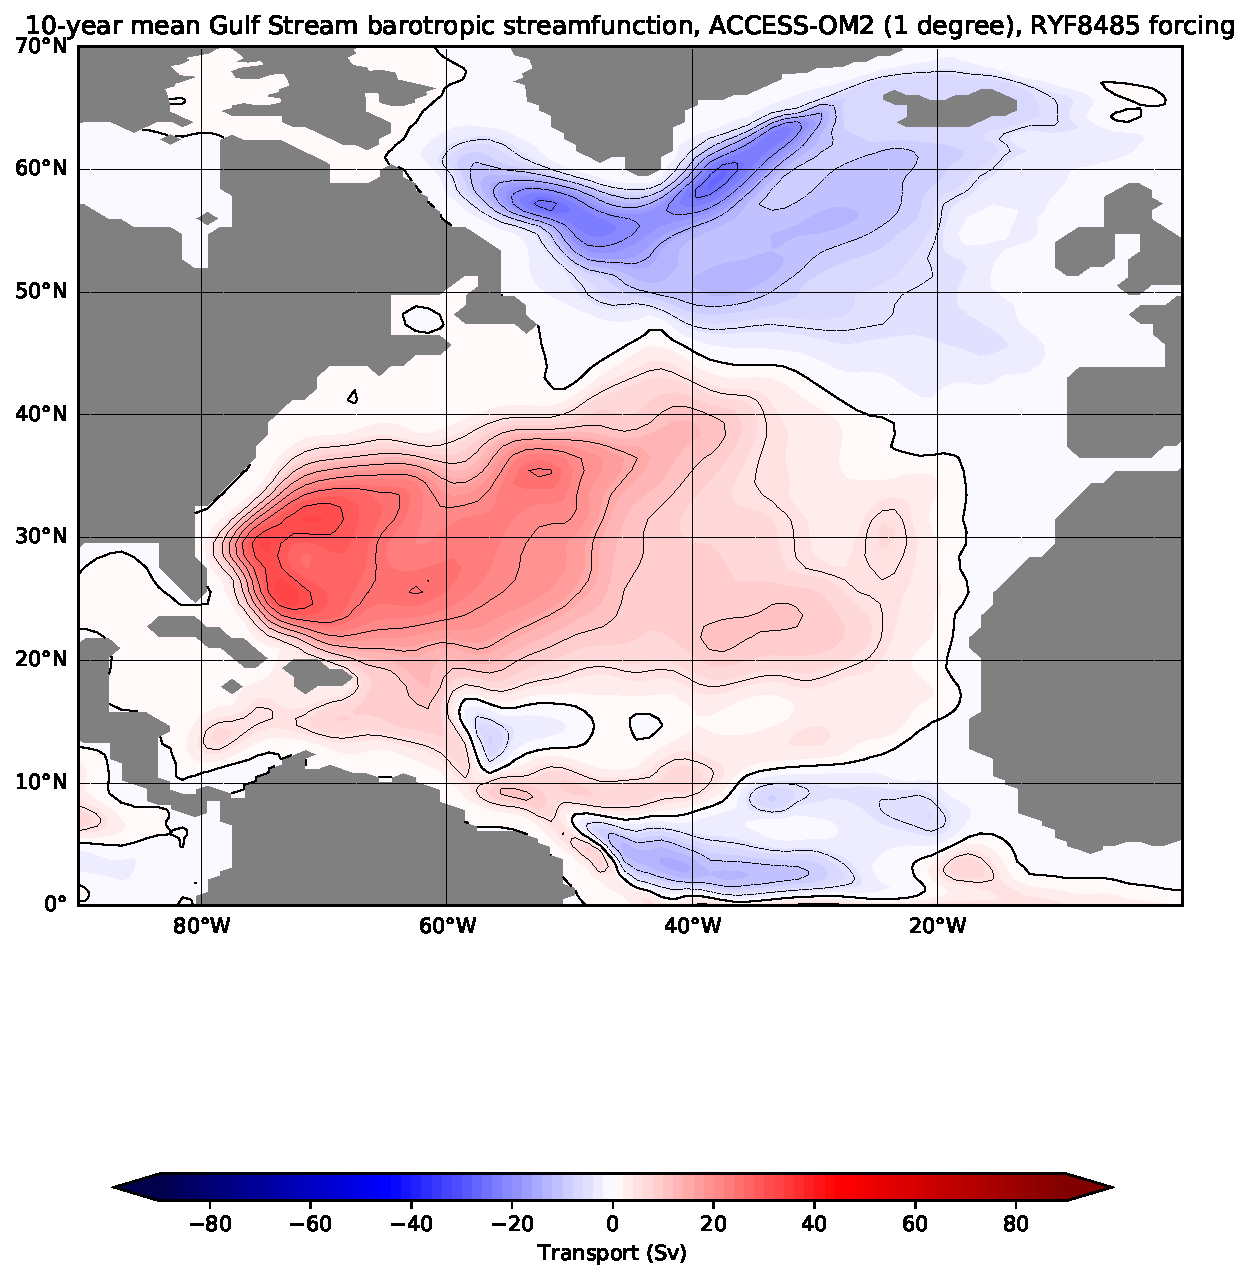
\includegraphics[width=.32\textwidth]{figures/BarotropicStreamfunction/GulfStream_transport_1deg.png}\hfill
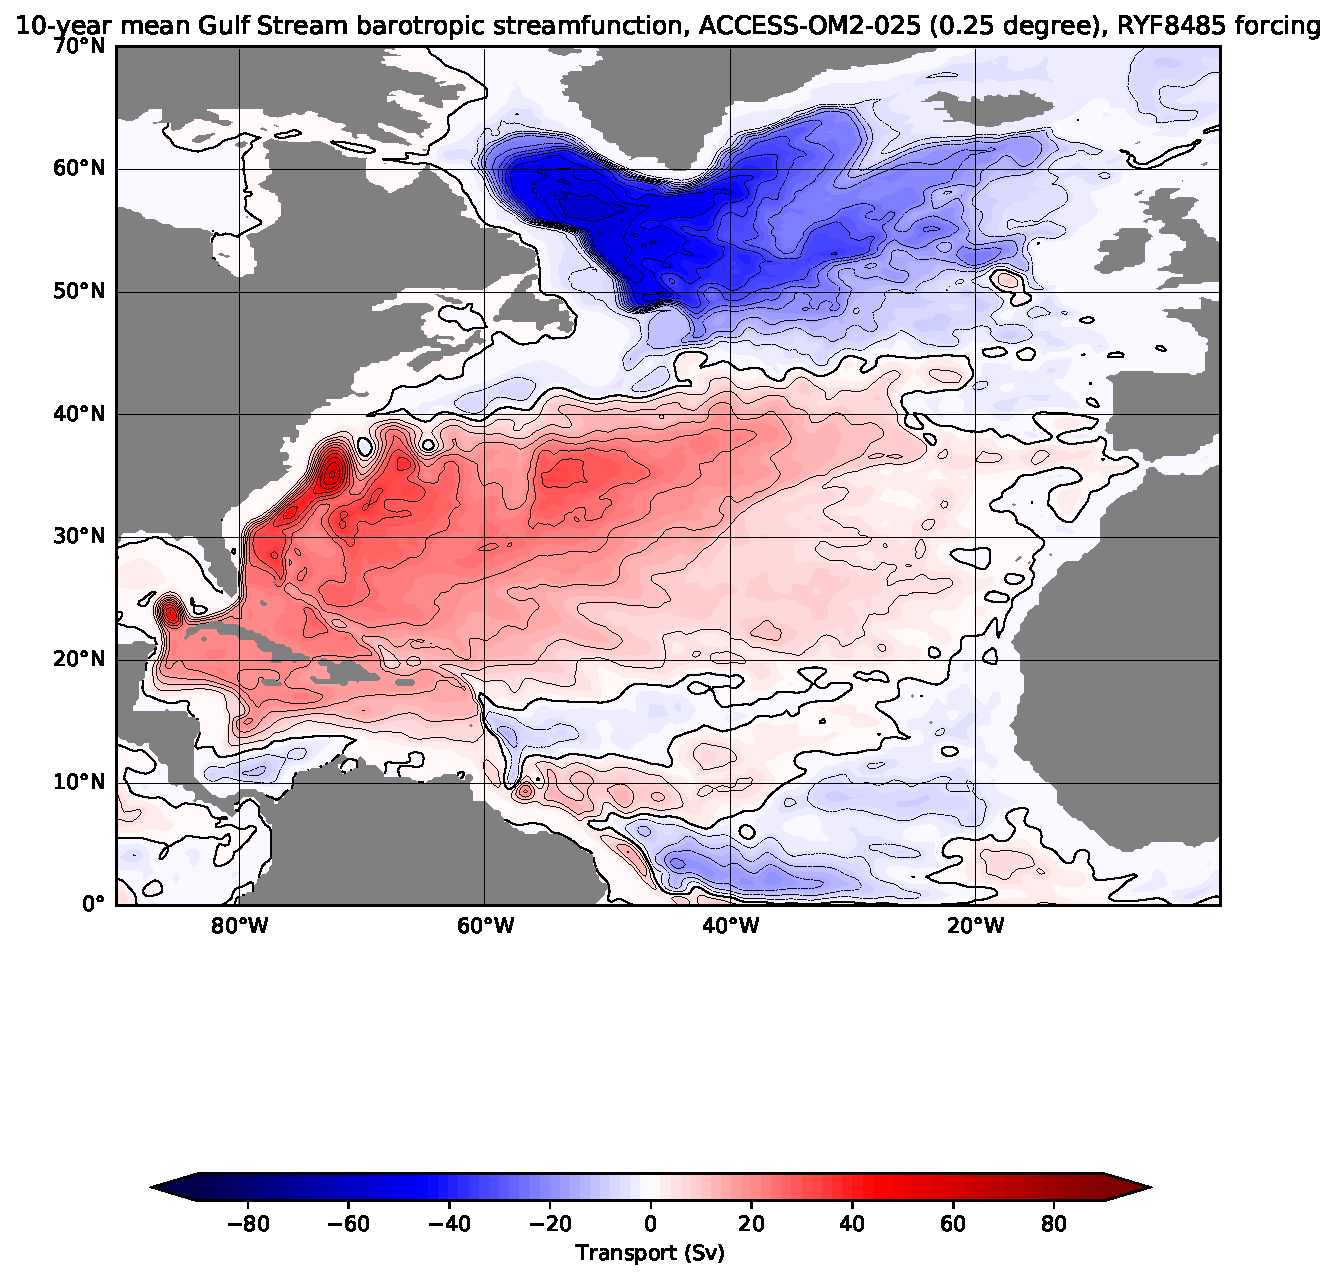
\includegraphics[width=.32\textwidth]{figures/BarotropicStreamfunction/GulfStream_transport_025deg.png}\hfill
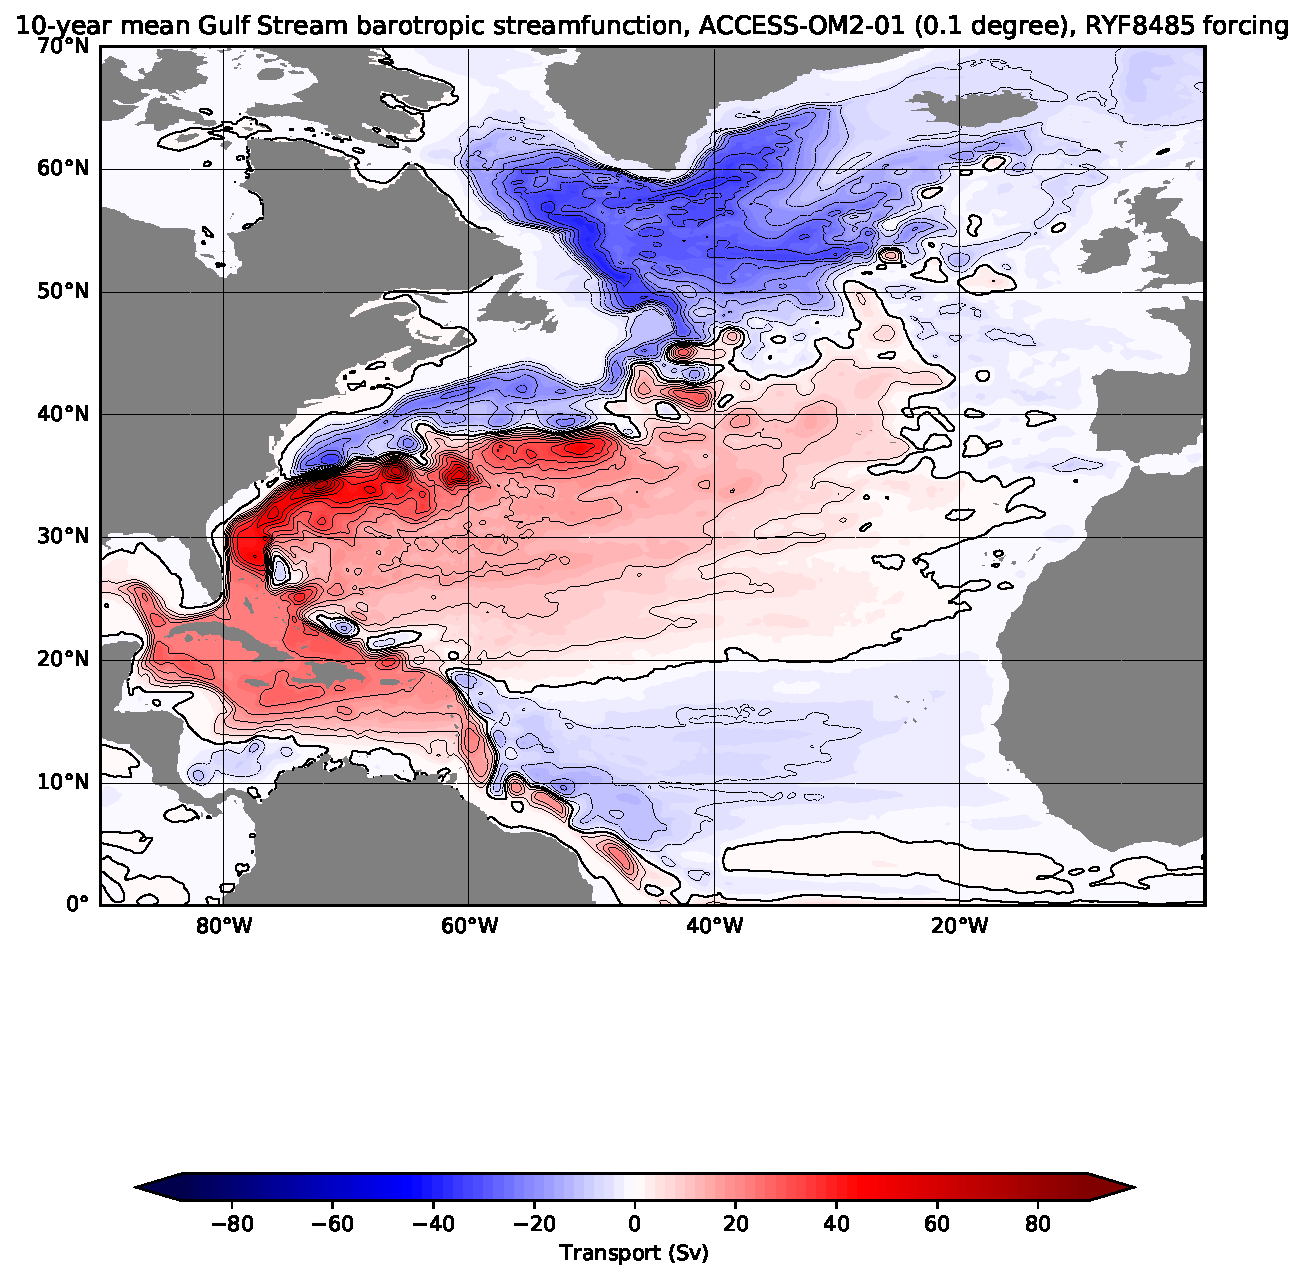
\includegraphics[width=.32\textwidth]{figures/BarotropicStreamfunction/GulfStream_transport_01deg.png}
\caption{Gulf Stream barotropic streamfunction for ACCESS-OM2 simulations. \TODO{Compare with \citet{ColindeVerdiereOllitrault2016a} figure 3:} \url{https://journals.ametsoc.org/na101/home/literatum/publisher/ams/journals/content/phoc/2016/15200485-46.1/jpo-d-15-0046.1/20160222/images/large/jpo-d-15-0046.1-f3.jpeg}}
\label{F:GulfStreamtransport}
\end{figure}


\subsection{Surface current speed and variability}
\citet{LaurindoMarianoLumpkin2017a}
\citet{ArcherRoughanKeatingSchaeffer2017a,ArcherShayJohns2017a,ArcherKeatingRoughanJohnsLumpkinBeron-VeraShay2018a}
\citet{WijeratnePattiaratchiProctor2018a}

See figures~\ref{F:EACsnap}--\ref{F:GulfStreamclim}.

Kuroshio separation is late in all models (figure~\ref{F:Kuroshioclim}). Suspect this is due to anomalous wind stress curl in norther Pacific under 8485RYF \TODO{check}.

Gulf Stream separation is poor at 0.25deg (figure~\ref{F:GulfStreamclim}).

\begin{figure}[htp]
\includegraphics[width=\textwidth]{figures/surface_current/EAC_snap.png}
\caption{East Australian Current surface speed from (a) observations \citep[1979--2015 mean from drifters at 15\,m;][]{LaurindoMarianoLumpkin2017a} and snapshots \FIXME{daily mean? what date?} from ACCESS-OM2 simulations at (b) 1$^\circ$ resolution; (c) 0.25$^\circ$ resolution and (d) 0.1$^\circ$ resolution.}
\label{F:EACsnap}
\end{figure}

\begin{figure}[htp]
\includegraphics[width=\textwidth]{figures/surface_current/Agulhas_snap.png}
\caption{Agulhas Current surface speed from (a) observations \citep[1979--2015 mean from drifters at 15\,m;][]{LaurindoMarianoLumpkin2017a} and snapshots \FIXME{daily mean? what date?} from ACCESS-OM2 simulations at (b) 1$^\circ$ resolution; (c) 0.25$^\circ$ resolution and (d) 0.1$^\circ$ resolution.}
\label{F:Agulhassnap}
\end{figure}

\begin{figure}[htp]
\includegraphics[width=\textwidth]{figures/surface_current/Kuroshio_snap.png}
\caption{Kuroshio surface speed from (a) observations \citep[1979--2015 mean from drifters at 15\,m;][]{LaurindoMarianoLumpkin2017a} and snapshots \FIXME{daily mean? what date?} from ACCESS-OM2 simulations at (b) 1$^\circ$ resolution; (c) 0.25$^\circ$ resolution and (d) 0.1$^\circ$ resolution.}
\label{F:Kuroshiosnap}
\end{figure}

\begin{figure}[htp]
\includegraphics[width=\textwidth]{figures/surface_current/GulfStream_snap.png}
\caption{Gulf Stream surface speed from (a) observations \citep[1979--2015 mean from drifters at 15\,m;][]{LaurindoMarianoLumpkin2017a} and snapshots \FIXME{daily mean? what date?} from ACCESS-OM2 simulations at (b) 1$^\circ$ resolution; (c) 0.25$^\circ$ resolution and (d) 0.1$^\circ$ resolution.}
\label{F:GulfStreamsnap}
\end{figure}

\begin{figure}[htp]
\includegraphics[width=\textwidth]{figures/surface_current/EAC_clim.png}
\caption{East Australian Current surface speed from (a) observations \citep[1979--2015 mean from drifters at 15\,m;][]{LaurindoMarianoLumpkin2017a} and climatology \TODO{over which years?} from ACCESS-OM2 simulations at (b) 1$^\circ$ resolution; (c) 0.25$^\circ$ resolution and (d) 0.1$^\circ$ resolution.}
\label{F:EACclim}
\end{figure}

\begin{figure}[htp]
\includegraphics[width=\textwidth]{figures/surface_current/Agulhas_clim.png}
\caption{Agulhas Current surface speed from (a) observations \citep[1979--2015 mean from drifters at 15\,m;][]{LaurindoMarianoLumpkin2017a} and climatology \TODO{over which years?} from ACCESS-OM2 simulations at (b) 1$^\circ$ resolution; (c) 0.25$^\circ$ resolution and (d) 0.1$^\circ$ resolution.}
\label{F:Agulhasclim}
\end{figure}

\begin{figure}[htp]
\includegraphics[width=\textwidth]{figures/surface_current/Kuroshio_clim.png}
\caption{Kuroshio surface speed from (a) observations \citep[1979--2015 mean from drifters at 15\,m;][]{LaurindoMarianoLumpkin2017a} and climatology \TODO{over which years?} from ACCESS-OM2 simulations at (b) 1$^\circ$ resolution; (c) 0.25$^\circ$ resolution and (d) 0.1$^\circ$ resolution.}
\label{F:Kuroshioclim}
\end{figure}

\begin{figure}[htp]
\includegraphics[width=\textwidth]{figures/surface_current/GulfStream_clim.png}
\caption{Gulf Stream surface speed from (a) observations \citep[1979--2015 mean from drifters at 15\,m;][]{LaurindoMarianoLumpkin2017a} and climatology \TODO{over which years?} from ACCESS-OM2 simulations at (b) 1$^\circ$ resolution; (c) 0.25$^\circ$ resolution and (d) 0.1$^\circ$ resolution.}
\label{F:GulfStreamclim}
\end{figure}


\subsection{Deep circulation}
\citet{OllitraultColindeVerdiere2014a}

\subsection{Transports through key straits and boundary currents}
See figure~\ref{F:StraitTransports}

See \citet[][figure J1]{GriffiesETAL2016a} for standard CMIP6/OMIP sections.

use zigzag method in tripolar region? - see appendix C4 in \citet{GriffiesETAL2016a}

\TODO{output vertical sections at high spatiotemporal resolution in diag\_table}

\begin{figure}[htp]
\includegraphics[width=\textwidth]{figures/strait_transports/strait_transports.pdf}
\caption{Transports through key straits. \TODO{fix Lombok, fix ranges, include 1 deg, label panels (a), (b) etc}}
\label{F:StraitTransports}
\end{figure}

\subsubsection{ITF}
\TODO{See ``Oc\'eane Richet - Indonesian Seas model assessment'' dir}

transports through straits - cf INSTANT array obs and 
\citet{SprintallWijffelsMolcardJaya2009a, HautalaSprintallPotemraChongPandoeBrayIlahude2001a}

Marsland 12 Apr 2018: ACCESS (1$^\circ$) used Rayleigh drag to shift transport from westernmost to easternmost strait to match obs. Also cf. 
Perth-Jakarta line (XBT?)

\subsubsection{Drake Passage}
\CONTRIBUTORS{Andy  Hogg}

Drake passage transport is about 135\,Sv at 0.1$^\circ$ resolution and about 105\,Sv 0.25$^\circ$ (see figure~\ref{F:StraitTransports}), \TODO{keep these up to date} significantly below the observed values of 173.3\,Sv \citep{DonohueTraceyWattsChidichimoChereskin2016a} and 175\,Sv \citep{ColindeVerdiereOllitrault2016a}.

\subsection{Equatorial current velocity and temperature structure}
\CONTRIBUTORS{Ryan Holmes}

See figure~\ref{F:eqPacific}.

cf. TOGA?

\begin{figure}[htp]
\includegraphics[width=\textwidth]{figures/equatorial_pacific/equatorial_pacific.pdf}
\caption[Equatorial Pacific temperature and currents]{Transects in the upper equatorial Pacific versus longitude at the Equator (left) and versus latitude at $220^\circ$E (right) for the model configurations \TODO{averaged over which years?} and observations from \citet{JohnsonSloyanKesslerMcTaggart2002a} \TODO{averaged over which years?} \TODO{check this is the correct reference}. Colours show temperature in $^\circ$C and white contours with black labels are eastward velocity isotachs (in cm\,s$^{-1}$; westward contours are dashed).}
\label{F:eqPacific}
\end{figure}



\subsection{Overturning}

The overturning circulation on density surfaces for all three resolutions is shown in Fig.~\ref{F:meanoverturning}.
This figure \ldots

\begin{figure}[ht]
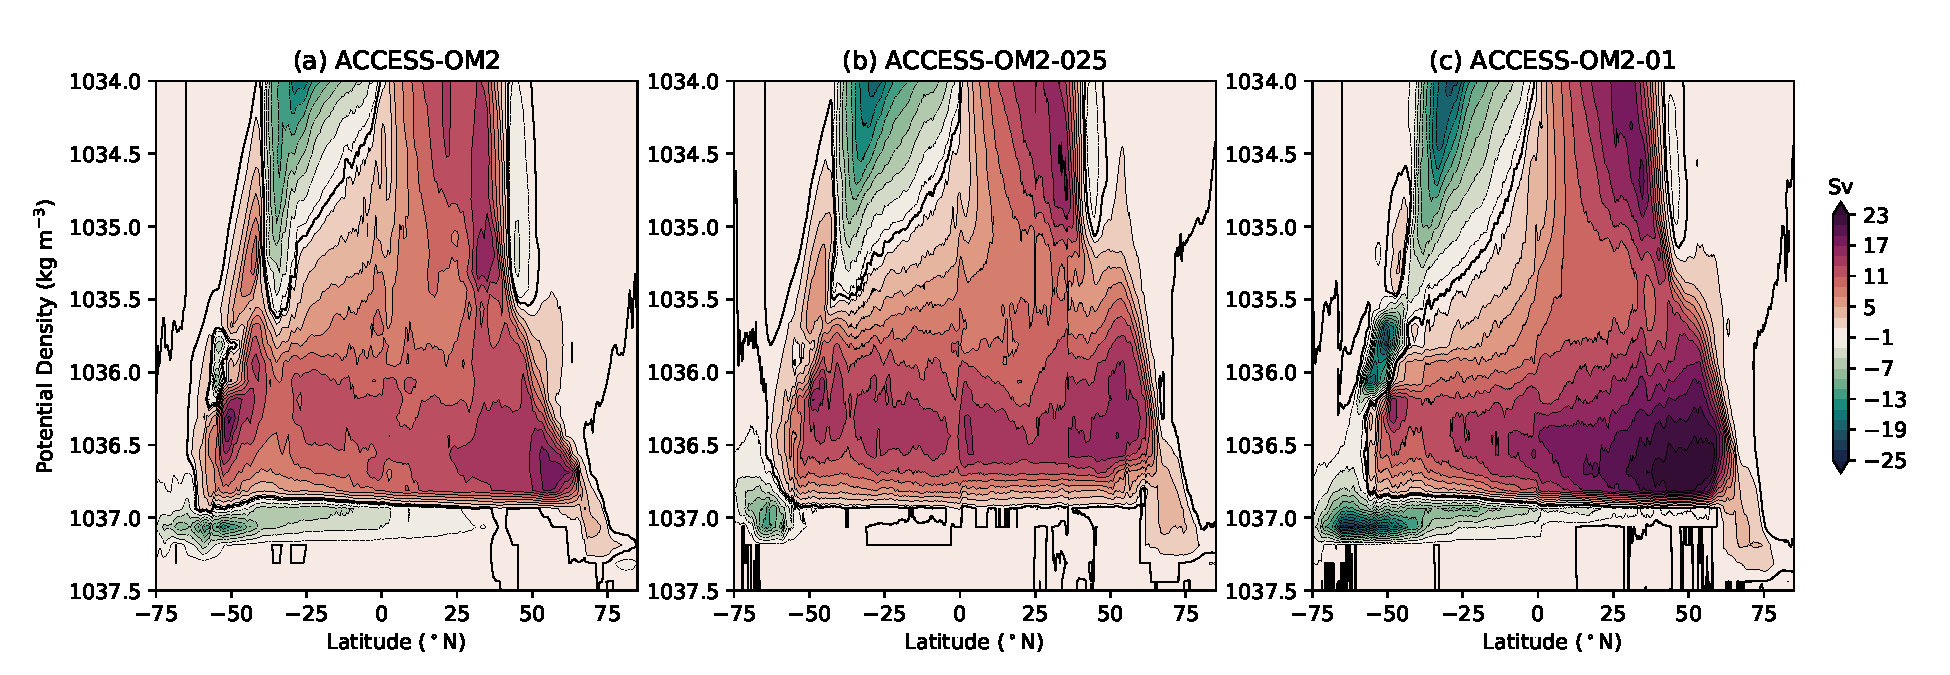
\includegraphics[width=\textwidth]{figures/overturning_circulation/mean_overturning.pdf}
\caption{Global overturning circulation on density surfaces ($\sigma_2$) for ACCESS-OM2 simulations at (a) 1$^\circ$ resolution; (b) 0.25$^\circ$ resolution and (c) 0.1$^\circ$ resolution.}
\label{F:meanoverturning}
\end{figure}


\citet{FarnetiDownesGriffiesMarslandBehrensBentsenBiBiastochBoning2015a}

\citet{LumpkinSpeer2007a}

\citet{Talley2013a}

\subsection{Meridional heat transport}
\CONTRIBUTORS{Ryan Holmes, Adele Morrison}

AMOC: do transect at 26.5N to cf RAPID array \url{http://www.rapid.ac.uk/rapidmoc/}
\citet{SmeedJoseyBeaulieuJohnsMoatFrajka-WilliamsRaynerMeinenBaringer2018a}

cf. \citet{NewsomBitzBryanAbernatheyGent2016a}? But this is just another model analysis?

Could also compare to reanalysis products, as done in \citet{GriffiesWintonAndersonBensonDelworthDufourDunneGoddardMorrison2015a}, Figure 7. \citet{Ganachaud2003} is another obs estimate to compare with.

\subsection{Model bias assessments}
Minimal model bias important for BOM for data assimilation in oceanMAPS, but is difficult to assess with repeat-year forcing as the mean of RYF is not climatology, so after many repeats of RYF the  slowly-adjusting ocean features will match neither climatology nor the state in the repeat year, even if the model itself is unbiased.
% -see  /Users/andy/Documents/COSIMA/COSIMA workshop 26-27 May 2016/Gary Brassington (BoM) Brassington_Ocean_modelling_and_forecasting_v3.pptx.pdf

cf BRAN

cf  \citet{KerryPowellRoughanOke2016a}

\subsection{Water mass properties and structure}
\CONTRIBUTORS{Adele Morrison}

mixed layer depth - CMIP5 models tend to underestimate winter MLD \citep{SalleeShuckburghBruneauMeijersBracegirdleWang2013a}.
\TODO{plot MLD and check to see that consistent definitions are used - see notebooks that compare model with IFREMER and MILA\_GPV obs}

see \citet{UotilaETAL2018a}

use Argo data

and MEOP southern ocean seal data \url{http://www.meop.net}?

\subsubsection{T/S diagrams}
\subsubsection{Deep water formation / transformation rates, locations, properties}
\citet{FarnetiDownesGriffiesMarslandBehrensBentsenBiBiastochBoning2015a}
\citet{AbernatheyCeroveckiHollandNewsomMazloffTalley2016a}
\citet{DownesGnanadesikanGriffiesSarmiento2011a}

\subsection{Heat conservation, bias and drift}
\CONTRIBUTORS{Chris Chapman, Ryan Holmes}

use XBT data from Chris Chapman?

cf FAFMIP? \citet{GregoryETAL2016a}

\subsubsection{SST bias}
WOA13v2 0.25-degree Arctic SST has spurious steps - see \url{https://github.com/OceansAus/access-om2/issues/103}

cf.\ SSTARS \citep{WijffelsETAL2018a}, available via \url{https://portal.aodn.org.au/}?

\subsubsection{lat/depth T sections and bias}
\subsubsection{Drift: depth/time T hovmollers}
\subsubsection{zonally averaged surface heat flux terms}

\subsection{Salt conservation, bias and drift}
cf FAFMIP? \citet{GregoryETAL2016a}
\subsubsection{SSS bias}
WOA13v2 0.25-degree Arctic SSS has spurious steps - see \url{https://github.com/OceansAus/access-om2/issues/103}
\subsubsection{lat/depth S sections and bias}
\subsubsection{Drift: depth/time S hovmollers}
\subsubsection{zonally averaged surface salt/freshwater flux terms}

\subsection{Variability}
\citet{DanabasogluYeagerKimBehrensBentsenBiBiastochBleckBoning2016a}
%\subsubsection{ENSO}
%\subsubsection{IOD}
%\subsubsection{SAM}
\subsubsection{Western boundary current variability}
\subsubsection{EKE spatial distribution and wavenumber spectrum}
\citet{OllitraultColindeVerdiere2014a}


also check EKE spectrum to see if it follows the expected slope - eg \citet{CapetMcWilliamsMolemakerShchepetkin2008a}
cf. spectrum obs: \citet{XuFu2011a}

\subsection{Sea level}
\citet{GriffiesYinDurackGoddardBatesBehrensBentsenBiBiastoch2014a}

\subsection{Sea ice}
see \citet{VaughanComisoAllisonCarrascoKaserKwokMoteMurrayPaul2013a, FlatoMarotzkeAbiodunBraconnotChouCollinsCoxDriouechEmori2013a}

problems comparing models to obs: \url{NotzHaumannHaakJungclausMarotzke2013a}

see \citet{Naughten2018a, NaughtenETAL2018a}

see \citet{NAS2017a}, \citet{HobbsMassomStammerjohnReidWilliamsMeier2016a, UotilaETAL2018a}

special issue: \url{https://agupubs.onlinelibrary.wiley.com/doi/toc/10.1002/(ISSN)2169-9291.NICE1}

see Kial's RYF sea ice assessment at 1deg

cf.\ ACCESS-OM \citep{UotilaOFarrellMarslandBi2012a, UotilaOFarrellMarslandBi2013a}

wavy ice features in 0.25deg --- poor EVP convergence? \url{https://github.com/OceansAus/access-om2/issues/87}

Too much ice south of Svalbard in 0.10deg --- \TODO{check Gulf Stream in 0.1deg --- is it carrying heat far enough north?}

\TODO{put probe points at narrowest point of northern Nares Str between Greenland and Ellesmere - compare ice export to \citet{KwokToudal-PedersenGudmandsenPang2010a}}

\TODO{summary plot of sea ice extent min and max contours for the 3 models and obs in NH and SH}

We have quite thick ice in small, isolated locations in some Arctic embayments (up to about 22m \TODO{check}) but at least it's not hundreds of metres as in \citet{DelworthRosatiAndersonAdcroftBalajiBensonDixonGriffiesLee2012a}.

Reanalyses for possible comparison with model (from Helen Beggs' email 21 Mar 2018):
\begin{itemize}
\item Reanalyses of sea ice observations: The OSI-SAF reanalysis is available in ~10 km resolution from:
\url{http://osisaf.met.no/p/ice/index.html#conc-reproc}
It covers the period from 1978 to 2009 with consistent algorithm processing. 
PUM and validation reports are available at the website as well.
OSI-SAF Daily sea ice concentration analyses are being ingested into the new Decadal OFAM Climate Model by Sakov and Sandery.
\item \url{http://osisaf.met.no}: ice concentration, edge, drift and emissivity on both hemispheres, as well as climate consistent time series
\item  Bremen/Hamburg University and their AMSR2 based products
\item NCEP (Bob Grumbine), \url{http://polar.ncep.noaa.gov/seaice/} - BoM uses NCEP 1/12$^\circ$ Daily Global Sea Ice Analyses as operational inputs into their SST analyses, used as the boundary condition to the NWP models
\end{itemize}

\url{http://psc.apl.uw.edu/research/projects/arctic-sea-ice-volume-anomaly/}


\TODO{check: are there katabatic winds in JRA55? if not, does this explain our lack of coastal polynyas? see \citet{ZhangVihmaStosselUotila2015a, StosselZhangVihma2011a}}
\TODO{Alex Fraser suggestion at AUV workshop: check formation rate -- is it just thin frazil in the model, so we actually do have coastal polynyas? could also look at category 1 ice thickness}

see Ice\_Validation\_ACCESS-OM2-01.ipynb \url{https://github.com/aekiss/cosima-cookbook/blob/master/notebooks/Ice_Validation_ACCESS-OM2-01.ipynb}
uses data from \url{http://nsidc.org}
%# TODO: update both to v3
%ObsDir = '/g/data/v45/akm157/data/NSIDC/NOAA_G02202_v2_conc_monthly/'  # from http://nsidc.org/data/G02202
%ObsDirExt = '/g/data/v45/akm157/data/NSIDC/NOAA_G02135_extent_monthly/'  # from http://nsidc.org/data/g02135

see SIMIP \citet{NotzJahnHollandHunkeMassonnetStroeveTremblayVancoppenolle2016a}
 
see \citet{ToyotaKimura2018a} - plastic rheology applies in MIZ

and check convergence \citet{BouillonFichefetLegatMadec2013a, KimmritzDanilovLosch2015a, LoschDanilov2012a, LemieuxTremblay2009a}

\citet{WangIlicakGerdesDrangeAksenovBaileyBentsenBiastochBozec2016a}

\citet{DownesFarnetiUotilaGriffiesMarslandBaileyBehrensBentsenBi2015a}

cf \citet{HeilMassomAllisonWorby2011a}
\ISSUE{3}
\subsubsection{Seasonal cycle of extent, coverage and thickness distribution}
\ISSUE{1}
\ISSUE{2}

Note that there are significant differences between passive microwave observational products \citep{IvanovaETAL2015a, RoachDeanRenwick2018a, MeierPengScottSavoie2014a} and \url{https://nsidc.org/support/faq/what-difference-between-nasa-team-algorithm-and-bootstrap-algorithm}
Sea ice extent is generally consistent, but sea ice area or concentration distributions differ significantly and this should be taken into account when assessing model performance \citep{RoachDeanRenwick2018a}.
\citet{NAS2017a}: `` As a general rule of thumb, said Dr. Massom, overall accuracies in ice concentration retrieval ranging from $\pm$5\% to $\pm$15\% are expected. Errors are largest in summer, over regions of predominantly thin/new ice, and year round in the marginal ice zone (MIZ) (up to $\pm$30\%) (Brucker et al., 2014; Comiso et al., 2011).''

NOAA/NSIDC Climate Data Record of Passive Microwave Sea Ice Concentration, Version 3 \citet{MeierFettererSavoieMalloryDuerrStroeve2017a, PengMeierScottSavoie2013a}, \url{http://nsidc.org/data/G02202}
This has a nominal resolution of 25\,km, considerably coarser than both the 0.25$^\circ$ and 0.1$^\circ$ models (table~\ref{T:hgrid}).
\TODO{show March and Sept ice concentration vs.\ obs} 
obs: 1988--1997 climatology from NOAA/NSIDC Climate Data Record of Passive Microwave Sea Ice Concentration, v3

Sea Ice Index, Version 3 \url{http://nsidc.org/data/g02135} 
See Figure~\ref{F:icevolumecategories}: the growth of Arctic ice volume is due to increasing category 5, presumably due to ridging.
We use \cice{kcatbound}=0, so lower bound of ice categories is 0, 0.64, 1.39, 2.47, 4.57m \citep[][table~2]{HunkeLipscombTurnerJefferyElliott2015a-CICE5p1}.
So by year 9 most of the ice volume (not area) is more than 4.57m thick, including in the summer minimum.

thickness: \url{http://psc.apl.uw.edu/sea_ice_cdr/}

Sea ice thickness and volume --- cf.\ IceSat data 2003--2008 \citep{KurtzMarkus2012a}

Compare thickness with cryosat data? - from late 2010 onwards \url{http://science-pds.cryosat.esa.int}
Or GIOMAS \citep[see][]{UotilaOFarrellMarslandBi2013a}? - though this is output from a data-assimilated model \citep{ZhangRothrock2003a} at about 1 degree resolution, monthly data  from 1/1979 to 12/2009 \url{http://psc.apl.washington.edu/zhang/Global_seaice/model.html} and \url{http://psc.apl.uw.edu/data/global-sea-ice-giomas-data-sets/}
Or \citet{WorbyGeigerPagetVan-WoertAckleyDeLiberty2008a}?
Or \citet{KwokCunningham2008a}?



\TODO{include maps of monthly mean concentration bias relative to passive microwave at the 3 resolutions: Sept and March in NH, Feb and Sept in SH}

\begin{figure}[ht]
\begin{center}
\includegraphics[height=0.3\textheight]{figures/ice_validation/1deg_concentration_map_NH_1990-1999_03_mean.png}\\
\includegraphics[height=0.3\textheight]{figures/ice_validation/025deg_concentration_map_NH_1990-1999_03_mean.png}\\
\includegraphics[height=0.3\textheight]{figures/ice_validation/01deg_concentration_map_NH_1990-1999_03_mean.png}
\end{center}
\caption[Arctic ice concentration maps, March]{Arctic sea ice concentration from the ACCESS-OM2 suite (left) and passive microwave (right), March mean.
Green (red) line is the 15\% concentration contour in the model (observations).
\TODO{make this more compact - no need to repeat obs 3 times}
}
\label{F:concentration_map_NH_March}
\end{figure}

\begin{figure}[ht]
\begin{center}
\includegraphics[height=0.3\textheight]{figures/ice_validation/1deg_concentration_map_NH_1990-1999_09_mean.png}\\
\includegraphics[height=0.3\textheight]{figures/ice_validation/025deg_concentration_map_NH_1990-1999_09_mean.png}\\
\includegraphics[height=0.3\textheight]{figures/ice_validation/01deg_concentration_map_NH_1990-1999_09_mean.png}
\end{center}
\caption[Arctic ice concentration maps, September]{Arctic sea ice concentration from the ACCESS-OM2 suite (left) and passive microwave (right), September mean.
Green (red) line is the 15\% concentration contour in the model (observations).
\TODO{make this more compact - no need to repeat obs 3 times}
}
\label{F:concentration_map_NH_Sept}
\end{figure}

\begin{figure}[ht]
\begin{center}
\includegraphics[height=0.3\textheight]{figures/ice_validation/1deg_concentration_map_SH_1990-1999_09_mean.png}\\
\includegraphics[height=0.3\textheight]{figures/ice_validation/025deg_concentration_map_SH_1990-1999_09_mean.png}\\
\includegraphics[height=0.3\textheight]{figures/ice_validation/01deg_concentration_map_SH_1990-1999_09_mean.png}
\end{center}
\caption[Antarctic ice concentration maps, September]{Antarctic sea ice concentration from the ACCESS-OM2 suite (left) and passive microwave (right), September mean.
Green (red) line is the 15\% concentration contour in the model (observations).
\TODO{make this more compact - no need to repeat obs 3 times}
}
\label{F:concentration_map_SH_Sept}
\end{figure}

\begin{figure}[ht]
\begin{center}
\includegraphics[height=0.3\textheight]{figures/ice_validation/1deg_concentration_map_SH_1990-1999_02_mean.png}\\
\includegraphics[height=0.3\textheight]{figures/ice_validation/025deg_concentration_map_SH_1990-1999_02_mean.png}\\
\includegraphics[height=0.3\textheight]{figures/ice_validation/01deg_concentration_map_SH_1990-1999_02_mean.png}
\end{center}
\caption[Antarctic ice concentration maps, February]{Antarctic sea ice concentration from the ACCESS-OM2 suite (left) and passive microwave (right), February mean.
Green (red) line is the 15\% concentration contour in the model (observations).
\TODO{make this more compact - no need to repeat obs 3 times}
}
\label{F:concentration_map_SH_Feb}
\end{figure}

%%%%%%%%%

\begin{figure}[ht]
\begin{center}
\includegraphics[height=0.23\textheight, bb = 461 0 923 505, clip]{figures/ice_validation/1deg_concentration_map_SH_1990-1999_02_mean.png}  % obs
\includegraphics[height=0.23\textheight, bb = 461 0 923 505, clip]{figures/ice_validation/1deg_concentration_map_SH_1990-1999_09_mean.png}\\  % obs
\includegraphics[height=0.23\textheight, bb = 0 0 461 505, clip]{figures/ice_validation/1deg_concentration_map_SH_1990-1999_02_mean.png}
\includegraphics[height=0.23\textheight, bb = 0 0 461 505, clip]{figures/ice_validation/1deg_concentration_map_SH_1990-1999_09_mean.png}\\
\includegraphics[height=0.23\textheight, bb = 0 0 461 505, clip]{figures/ice_validation/025deg_concentration_map_SH_1990-1999_02_mean.png}
\includegraphics[height=0.23\textheight, bb = 0 0 461 505, clip]{figures/ice_validation/025deg_concentration_map_SH_1990-1999_09_mean.png}\\
\includegraphics[height=0.23\textheight, bb = 0 0 461 505, clip]{figures/ice_validation/01deg_concentration_map_SH_1990-1999_02_mean.png}
\includegraphics[height=0.23\textheight, bb = 0 0 461 505, clip]{figures/ice_validation/01deg_concentration_map_SH_1990-1999_09_mean.png}
\end{center}
\caption[Antarctic ice concentration maps]{Antarctic monthly mean sea ice concentration from passive microwave observations (top) and ACCESS-OM2 at three resolutions (rows 2--4) for February (left) and September (right). 
The colour scale is nonlinear.
The green (red) line is the 15\% concentration contour in the model (observations).
}
\label{F:concentration_map_SH_Feb}
\end{figure}


%\end{document} %%%%%%%%%%%%%%%

\begin{figure}[ht]
\begin{center}
\includegraphics[height=0.21\textheight]{figures/ice_validation/ice_volume_min_mean_max_all.pdf}\\
\includegraphics[height=0.21\textheight]{figures/ice_validation/ice_volume_categories_cumulative1deg.pdf}\\
\includegraphics[height=0.21\textheight]{figures/ice_validation/ice_volume_categories_cumulative025deg.pdf}\\
\includegraphics[height=0.21\textheight]{figures/ice_validation/ice_volume_categories_cumulative01deg.pdf}
\end{center}
\caption[Sea ice volume timeseries.]{Sea ice volume timeseries in the different configurations. 
Top row: running 12-month minimum, mean and maximum.
Remaining rows: breakdown of ice volume by category (thick lines show the 12-month running mean).
Lower bound of ice thickness categories is 0, 0.64, 1.39, 2.47, 4.57m.
\TODO{use a common scale for the category plots in each hemisphere}
}
\label{F:icevolumecategories}
\end{figure}

Sea ice extent --- see \citet{IvanovaGlecklerTaylorDurackMarvel2016a}


\begin{figure}[ht]
\includegraphics[width=\textwidth]{figures/ice_validation/ice_extent.pdf}
\caption{Seasonal cycle of ice extent at 0.1$^\circ$ resolution \FIXME{averaged over which years?} compared to 1979--1998 climatology of NOAA/NSIDC G02135 Sea Ice Index v3 (\url{http://nsidc.org/data/g02135}) \TODO{show all resolutions}
\TODO{check that model extent is correctly calculated --- total area in which ice cover exceeds 15\%?}
}
\label{F:iceextent}
\end{figure}

\subsubsection{Age}
\subsubsection{Formation rate}
ice production rate in coastal polynyas \citep{TamuraOhshimaNihashi2008a,TamuraOhshima2011a,TamuraOhshimaFraserWilliams2016a,NihashiOhshima2015a,OhshimaNihashiIwamoto2016a}
- see Adele's email 9 Mar 2018 - includes a script and netcdf version.
Looks like you can download the data set here:
\url{http://www.lowtem.hokudai.ac.jp/wwwod/polar-seaflux/}
what diagnostics give us production in CICE? f_congel gives basal growth -- not relevant?
meltb, meltl,melts, meltt?
frazil?



\subsubsection{Drift}
cf.\ Kimura ice motion dataset - 60km
Petra is getting a 30km dataset

\citet{GilesMassomHeilHyland2011a}
\citet{SumataETAL2014a, SumataKwokGerdesKaukerKarcher2015a, SumataGerdesKaukerKarcher2015a, SzanyiLukovichBarberHaller2016a}
\citet{KwokPangKacimi2017a} % data in /Users/andy/Documents/Eprints/KwokPangKacimi2017a/KwokPangKacimi2017a-data-82_13_imv_iceedge

\subsubsection{Ice deformation}
cf. \citet{HutchingsRobertsGeigerRichter-Menge2011a}

\subsubsection{Polynyas}
How good are katabatic winds in JRA55? cf.\ polar WRF?

\citet{UotilaOFarrellMarslandBi2013a}
\citet{GirardWeissMolinesBarnierBouillon2009a}
\citet{KwokHunkeMaslowskiMenemenlisZhang2008a}

\FloatBarrier

\subsection{Particularly important regions}
Pick locations with detailed obs records for regional studies

\subsubsection{ACC}
\citet{Rintoul2018a}

cf SOSE \citet{MazloffHeimbachWunsch2010a}

transport

EKE
\citet{FarnetiDownesGriffiesMarslandBehrensBentsenBiBiastochBoning2015a}

\subsubsection{Antarctic margins}
\CONTRIBUTORS{Adele Morrison}

dense water formation
dense water transport down slope

\subsubsection{East Australian Current}
\citet{LaurindoMarianoLumpkin2017a}
\citet{ArcherRoughanKeatingSchaeffer2017a, ArcherShayJohns2017a, ArcherKeatingRoughanJohnsLumpkinBeron-VeraShay2018a}
\citet{WijeratnePattiaratchiProctor2018a}
\citet{ZilbermanRoemmichGilleGilson2018a, ZilbermanRoemmichGille2014a}
\citet{FengZhangOkeMonselesanChamberlainMatearSchiller2016a}

\url{http://www.clivar.org/clivar-panels/pacific/spice}

\subsubsection{Leeuwin Current}
\citet{WijeratnePattiaratchiProctor2018a}
\citet{FengZhangOkeMonselesanChamberlainMatearSchiller2016a}

\subsubsection{North Atlantic}
North Atlantic mean state \citet{DanabasogluYeagerBaileyBehrensBentsenBiBiastochBoningBozec2014a}
and variability \citet{DanabasogluYeagerKimBehrensBentsenBiBiastochBleckBoning2016a}

\subsubsection{Arctic Ocean / Greenland-Iceland-Norway (GIN) Seas}

cf. \citet{BehrendtSumataRabeSchauer2018a} \url{https://doi.pangaea.de/10.1594/PANGAEA.872931}?

mixed layer depth

water properties

bottom water formation

bottom water transport over sills

\citet{WangIlicakGerdesDrangeAksenovBaileyBentsenBiastochBozec2016b}
\citet{IlicakDrangeWangGerdesAksenovBaileyBentsenBiastochBozec2016a}

\subsubsection{Pacific}
\citet{TsengLinChenThompsonBentsenBoningBozecCassouChassignet2016a}

\subsubsection{Agulhas}
transport, structure, variability, leakage
 
 
\section{Things to fix for next time}

\subsection{For all resolutions}
\begin{itemize}
\item Make cice output more like SIMIP \citep{NotzJahnHollandHunkeMassonnetStroeveTremblayVancoppenolle2016a}
\item Fix calendar \url{https://github.com/OceansAus/access-om2/issues/117}
\item Use WOA2018 for initial condition and salt restoring? \url{https://www.nodc.noaa.gov/OC5/woa18/} --- but still has discontinuities and noise in Arctic surface salinity
\item As recommended by \citet{TsujinoETAL2018a}, for consistency with JRA55-do, use \citet{Gill82a} formulas instead of \citet{LargeYeager2004a,LargeYeager2009a}
\end{itemize}


\subsection{At 0.1 degree}
Easy things:
\begin{itemize}
\item Use non-mushy ice thermodynamics for speed
\item Set min_thick to the top level thickness in bathymetry: \url{https://github.com/OceansAus/access-om2/issues/99}
\item Use Nic's bathymetry with Severny Island seamounts removed
\item Fill in very fine bathymetry near tripoles? - this could allow reduction in ndtd
\item Fix salt restoring file \url{https://github.com/OceansAus/access-om2/issues/74}
\item Use explicit vertical diffusivity (e.g.\ \mom{background_diffusivity} = $\SI{1e-6}{m^2s^{-1}}$, spatially uniform) --- may improve (thicken) thermocline in equatorial Pacific and Indonesian seas?
\item Use conservative temperature
\item Output vorticity at only one depth
\item Make cice output more compact - don't output grid data every day
\item Try increased lateral viscosity to reduce vorticity noise \url{https://github.com/OceansAus/access-om2/issues/107}
\item Rayleigh friction at northern end of Novaya Zemlya?
\item Improve efficiency:
\begin{itemize}
\item Either increase dt (check that vorticity doesn't get noisy) or reduce ndtd
\item Improve load balance: roundrobin/sectrobin, experiment with block sizes and NTASK
\end{itemize}
\item experiment with EAP? \citet{Naughten2018a} found it improved things
\end{itemize}

Harder things:
\begin{itemize}
\item Sort out noise in surface vertical tracer diffusion \url{https://github.com/OceansAus/access-om2/issues/110}
\item Fix bug at tripole seam \url{https://github.com/OceansAus/access-om2/issues/86}
\item Move tripoles further from ocean to increase minimum cell size
\end{itemize}
 
 \section{Acknowledgments}
Model development has been partly funded by ARC Linkage grant LP160100073.
Runs were undertaken on the NCI National Facility in Canberra, which is supported by the Australian Commonwealth Government.

\appendix
\section{Auto-generated namelists}

\rowcolors{1}{lightblue}{white}

% \newcommand{\nmldiffer}[1]{#1} % no special display of differing variables
%\newcommand{\nmldiffer}[1]{\textbf{#1}} % bold display of differing variables
\definecolor{hilite}{cmyk}{0, 0, 0.9, 0}\renewcommand{\nmldiffer}[1]{\colorbox{hilite}{#1}}\setlength{\fboxsep}{0pt} % colour highlight of differing variables (requires color package)
\renewcommand{\nmllink}[2]{#1} % don't link variables
% \newcommand{\nmllink}[2]{\href{https://github.com/mom-ocean/MOM5/search?q=#2}{#1}} % link variables to documentation (requires hyperref package)
%\newcommand{\nml}[1]{{\small\textsf{\input{local/#1}}}} % use nml tables generated from local files
%\renewcommand{\nml}[1]{{\small\textsf{\input{raijin/#1}}}} % use nml tables generated on raijin
\renewcommand{\nml}[1]{{\small\textsf{\input{namelists/#1}}}} % use nml tables from raijin mirror
%\newlength{\nmllen}\setlength{\nmllen}{13ex}

These are auto-generated by make\_nml\_tables.py which uses nmltab (\url{https://github.com/aekiss/nmltab}).
Variables are weblinks to source code searches. 
Variables that differ between the models are \nmldiffer{\textcolor{link}{highlighted}}.
\ignored{Greyed values} are ignored. % (greying only works in groups with use_this_module shown, so typically doesn't work for tables of differences).

\TODO{generate complete tables that include the default values of parameters not specified in namelists}

\rowcolors{1}{lightblue}{white}
%\setlength{\nmllen}{18ex} % works well for 3 columns
\setlength{\nmllen}{13ex} % works well for 4 columns

\subsection{MOM namelist `input.nml'}\label{S:mom-namelist}
%\renewcommand{\nmllink}[2]{\href{https://github.com/mom-ocean/MOM5/search?q=#2}{#1}} % link to documentation (requires hyperref package)
%\renewcommand{\nmllink}[2]{\hypertarget{mom:#2}{\href{https://github.com/mom-ocean/MOM5/search?q=#2}{#1}}} % link to documentation (requires hyperref package)
\renewcommand{\nmllink}[2]{\hexhypertarget{mom:#2}{\href{https://github.com/mom-ocean/MOM5/search?q=#2}{#1}}} % link to documentation (requires hyperref package)
\nml{input_nml.tex}

\subsection{CICE namelists}\label{S:cice-namelist}
See \url{https://ncar.github.io/CICE/users_guide/ice_nml_var.html}.
%\renewcommand{\nmllink}[2]{\href{https://github.com/OceansAus/cice5/search?q=#2}{#1}} % link to documentation (requires hyperref package)
\renewcommand{\nmllink}[2]{\hexhypertarget{cice:#2}{\href{https://github.com/OceansAus/cice5/search?q=#2}{#1}}} % link to documentation (requires hyperref package)
\subsubsection{cice\_in.nml}
\nml{cice_in_nml.tex}
\subsubsection{input\_ice.nml}
\nml{input_ice_nml.tex}
\subsubsection{input\_ice\_gfdl.nml}
\nml{input_ice_gfdl_nml.tex}
\subsubsection{input\_ice\_monin.nml}
\nml{input_ice_monin_nml.tex}

\subsection{YATM namelist `atm.nml'}\label{S:yatm-namelist}
%\renewcommand{\nmllink}[2]{\href{https://github.com/OceansAus/libaccessom2/search?q=#2}{#1}} % link to documentation (requires hyperref package)
\renewcommand{\nmllink}[2]{\hexhypertarget{yatm:#2}{\href{https://github.com/OceansAus/libaccessom2/search?q=#2}{#1}}} % link to documentation (requires hyperref package)
\nml{atm_nml.tex}

%\subsection{MATM namelist `input\_atm.nml'}\label{S:matm-namelist}
%\renewcommand{\nmllink}[2]{\href{https://github.com/OceansAus/matm/search?q=#2}{#1}} % link to documentation (requires hyperref package)
%\nml{input_atm_nml.tex}

\section{Auto-generated tables of namelist changes within runs}
\TODO{do this}
%\renewcommand{\nmldiffer}[1]{#1} % no special display of differing variables
%\runchanges{access-om2-01/01deg_jra55v13_ryf8485_spinup1}
%\runchanges{access-om2-01/01deg_jra55v13_ryf8485_spinup2}
%\runchanges{access-om2-01/01deg_jra55v13_ryf8485_spinup3}
%\runchanges{access-om2-01/01deg_jra55v13_ryf9091_spinup1}
%\runchanges{access-om2-025/025deg_jra55_ryf_broadwell_test}
%\runchanges{access-om2-025/025deg_jra55_ryf_spinup1}
%\runchanges{access-om2-025/025deg_jra55_ryf_spinup2}
%\runchanges{access-om2-025/025deg_jra55_ryf_spinup3}
%\runchanges{access-om2-025/025deg_jra55_ryf_spinup4}
%\runchanges{access-om2-025/025deg_jra55_ryf_spinup5}
%\runchanges{access-om2-025/025deg_jra55_ryf_spinup6}
%\runchanges{access-om2-025/025deg_jra55_ryf_spinup7}
%\runchanges{access-om2-025/025deg_jra55_ryf_spinup7_RCP45}
%\runchanges{access-om2-025/025deg_jra55v13_ryf8485_gmredi}
%\runchanges{access-om2-025/025deg_jra55v13_ryf8485_redi}
%\runchanges{access-om2-025/025deg_jra55v13_ryf8485_redi2}
%\runchanges{access-om2-025/025deg_jra55v13_ryf8485_redi3}
%\runchanges{access-om2-025/025deg_jra55v13_ryf8485_spinup_A}
%\runchanges{access-om2/1deg_core_nyf_spinup_A}
%\runchanges{access-om2/1deg_jra55_ryf8485_spinup1}
%\runchanges{access-om2/1deg_jra55_ryf8485_spinup2}
%\runchanges{access-om2/1deg_jra55_ryf_RCP45}
%\runchanges{access-om2/1deg_jra55_ryf_spinup1}
%\runchanges{access-om2/1deg_jra55_ryf_spinup2}
%\runchanges{access-om2/1deg_jra55_ryf_spinup3}
%\runchanges{access-om2/1deg_jra55_ryf_spinup4}
%\runchanges{access-om2/1deg_jra55_ryf_spinup5}
%\runchanges{access-om2/1deg_jra55_ryf_spinup6}
%\runchanges{access-om2/1deg_jra55_ryf_spinup7}
%\runchanges{access-om2/1deg_jra55_ryf_spinup8}
%\runchanges{access-om2/1deg_jra55_ryf_spinup9}
%\runchanges{access-om2/1deg_jra55v13_ryf0304_RCP45}
%\runchanges{access-om2/1deg_jra55v13_ryf0304_spinup_A}
%\runchanges{access-om2/1deg_jra55v13_ryf8485_RCP45}
%\runchanges{access-om2/1deg_jra55v13_ryf8485_spinup_A}
%\runchanges{access-om2/1deg_jra55v13_ryf9091_RCP45}
%\runchanges{access-om2/1deg_jra55v13_ryf9091_spinup_A}

\section{Auto-generated tables of namelist differences from ACCESS, ACCESS-CM2, ACCESS-ESM, OFAM3}\label{S:namelist-model-comparisons}

\subsection{ACCESS-OM2-01 MOM compared to OFAM3}
Only differences are shown.
\renewcommand{\nmldiffer}[1]{#1} % no special display of differing variables
\renewcommand{\nmllink}[2]{\href{https://github.com/mom-ocean/MOM5/search?q=#2}{#1}} % link to documentation (requires hyperref package)
\nml{OFAM3_input_nml.tex}

\subsection{ACCESS-OM2-01 MOM compared to MOM-SIS-01 and GFDL}

\subsection{ACCESS-OM2-01 CICE compared to RASM and NCAR}\label{S:rasm-namelist}

ice_in_RASM  \TODO{get permisssion}

ncar_ice_in  \TODO{get permisssion}

\setlength{\parskip}{0em}
\bibliographystyle{ametsoc2014}
\bibliography{ACCESS-OM2-1-025-010deg}

\end{document}  
